
The methods presented in the previous chapter result in a model for studying viruses that incorporates the spatial spread of virus, has the ability to produce simulations in seconds, and has the flexibility to be applied to real data. In this chapter, the accuracy, speed, and applicability of the model is presented. I will show accurate simulations of plaque assays, the speed increase of the simulations by GPUs, and the analysis of virus infections.

\section{Model simulation}

Using the influenza parameters of table \ref{tab_params}, I simulated infections initiated with 1001365 cells in a dish, of which 100 randomly chosen cells are infected and no initial virus. Figure \ref{fig_FullDish_cellandvirus} shows different views of plaques forming in the entire dish. On the left are cells in the different stages of infection described in section \ref{ABM}, where the healthy cells are colored green, eclipse cells are colored cyan, infected cells are colored red, and dead cells are colored black. On the right are figures showing the corresponding virus concentrations that are over the cells, where areas of higher concentration are colored yellow and areas of lower concentration are colored purple. Figure \ref{fig_FullDish_cellandvirus} shows the infection in 5 hour increments starting at 5 hours, when no cells are producing virus, and ending at 60 hours, when almost all the cells have died. The ABM reproduces the plaques typically seen in experimental \emph{in vitro} infections \citep{holder11H274Y}. 

\begin{figure}
\centering
\begin{minipage}{0.8\linewidth}
\centering
\begin{multicols}{2}
    \resizebox{0.48\textwidth}{!}{%
        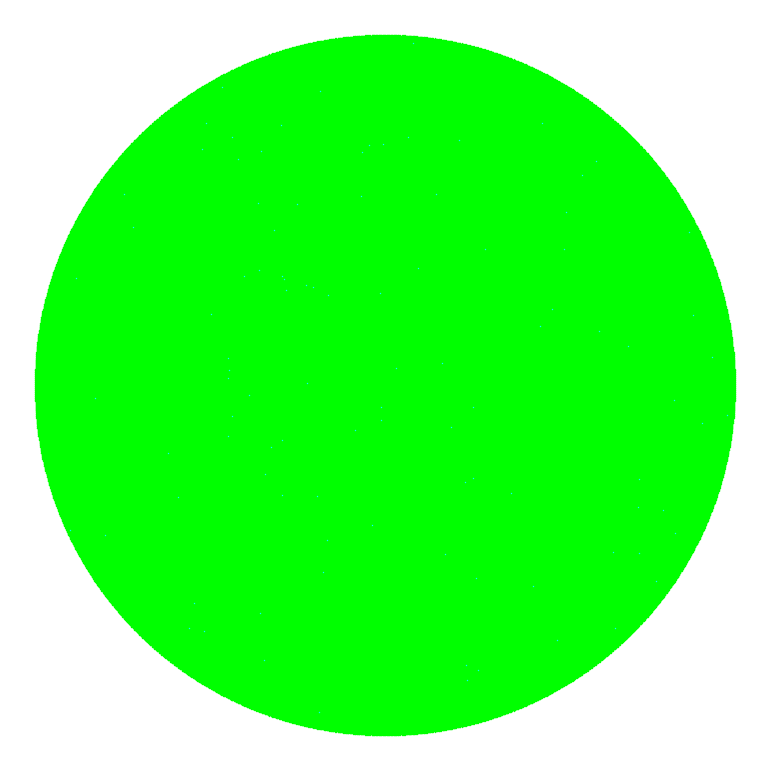
\includegraphics[width=0.48\textwidth]{Figures/Full-Dish-CellPhotos/cell9.png}
        
\includegraphics[width=0.48\textwidth]{Figures/Full-Dish-VirusPhotos/virus9.png}}

    \resizebox{0.48\textwidth}{!}{%
        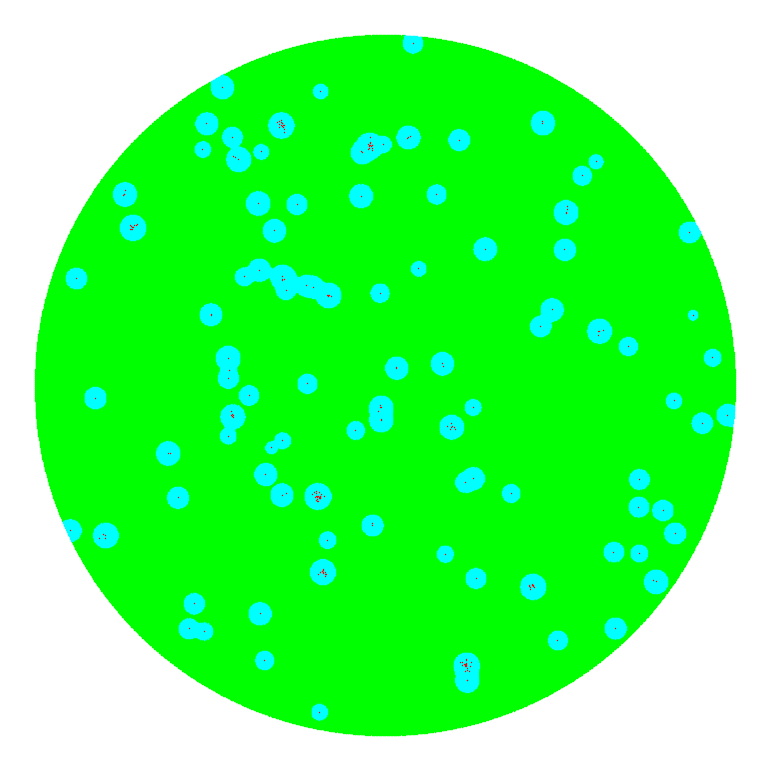
\includegraphics[width=0.48\textwidth]{Figures/Full-Dish-CellPhotos/cell19.png}
        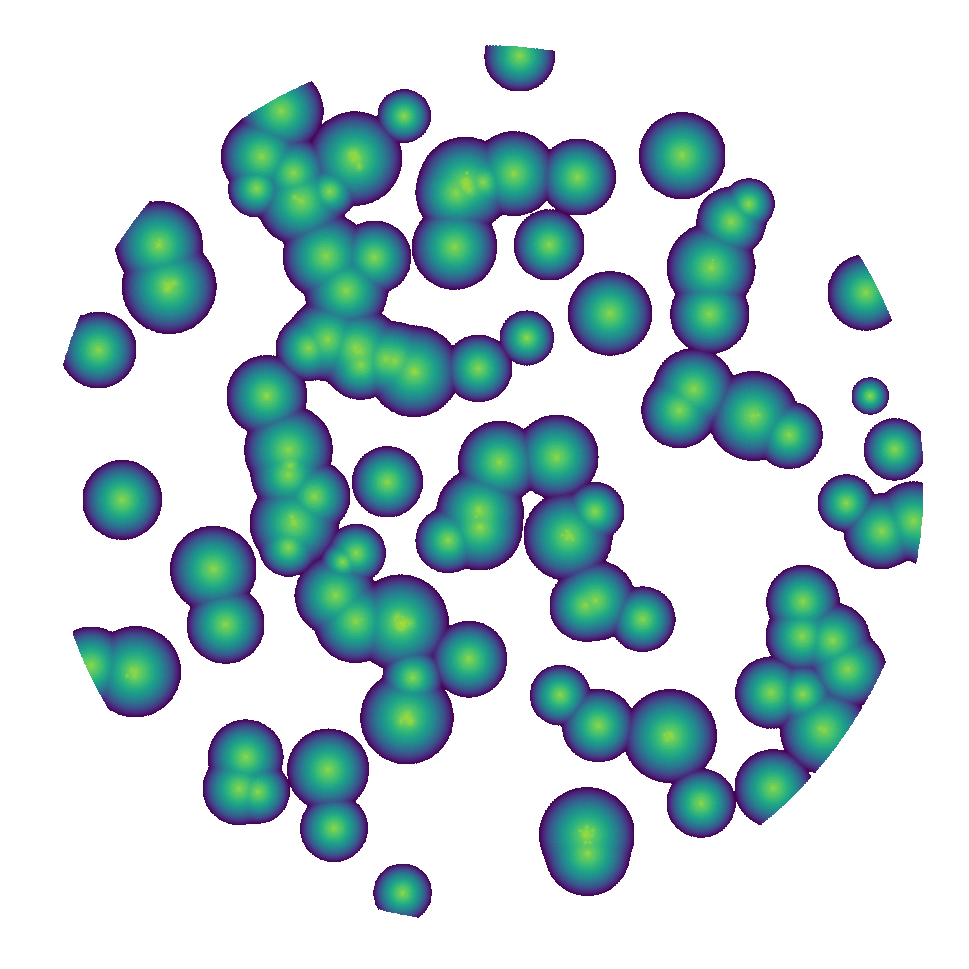
\includegraphics[width=0.48\textwidth]{Figures/Full-Dish-VirusPhotos/virus19.png}}

    \resizebox{0.48\textwidth}{!}{%
        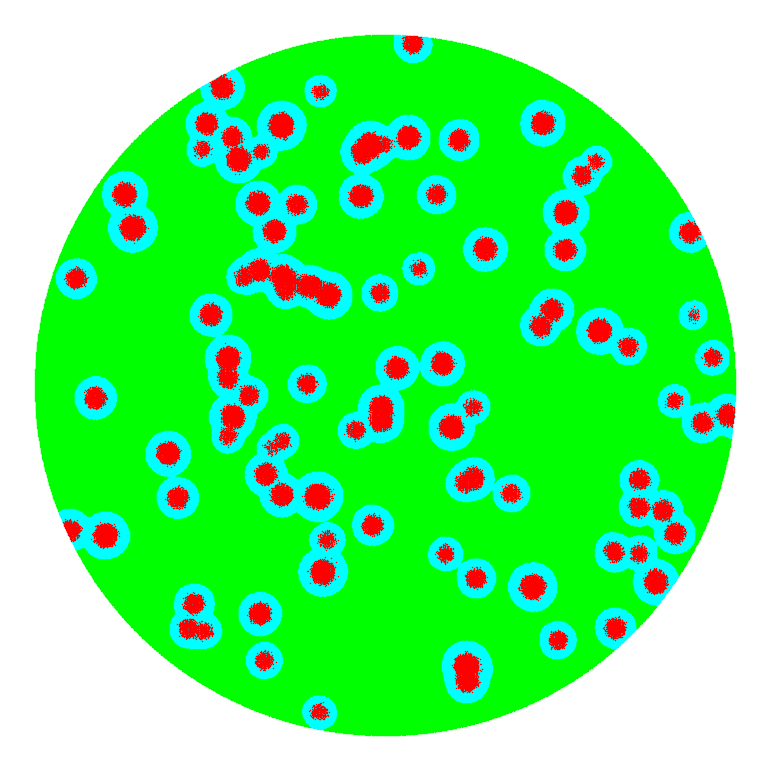
\includegraphics[width=0.48\textwidth]{Figures/Full-Dish-CellPhotos/cell29.png}
        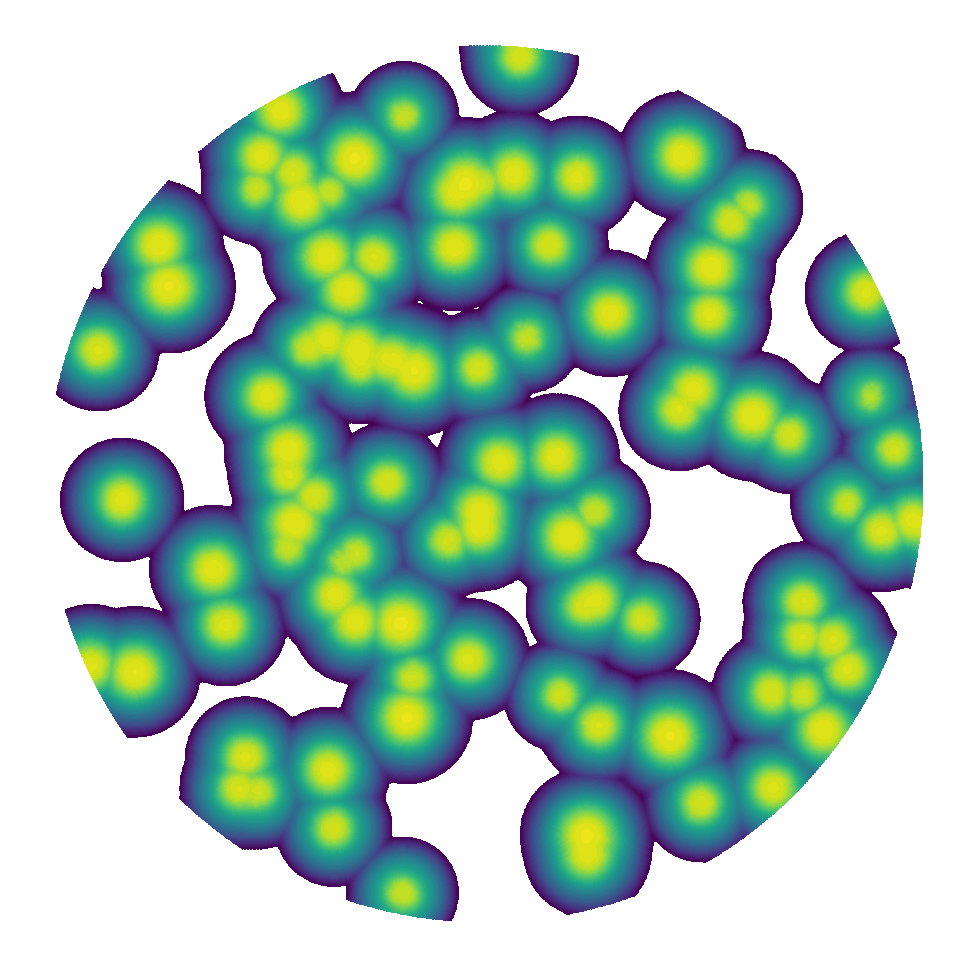
\includegraphics[width=0.48\textwidth]{Figures/Full-Dish-VirusPhotos/virus29.png}}

    \resizebox{0.48\textwidth}{!}{%
        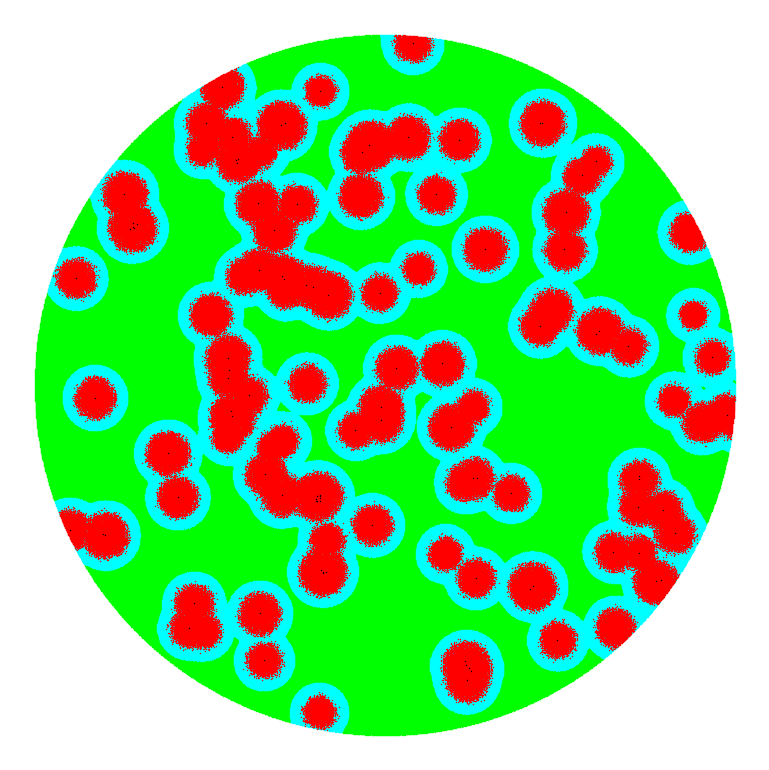
\includegraphics[width=0.48\textwidth]{Figures/Full-Dish-CellPhotos/cell39.png}
        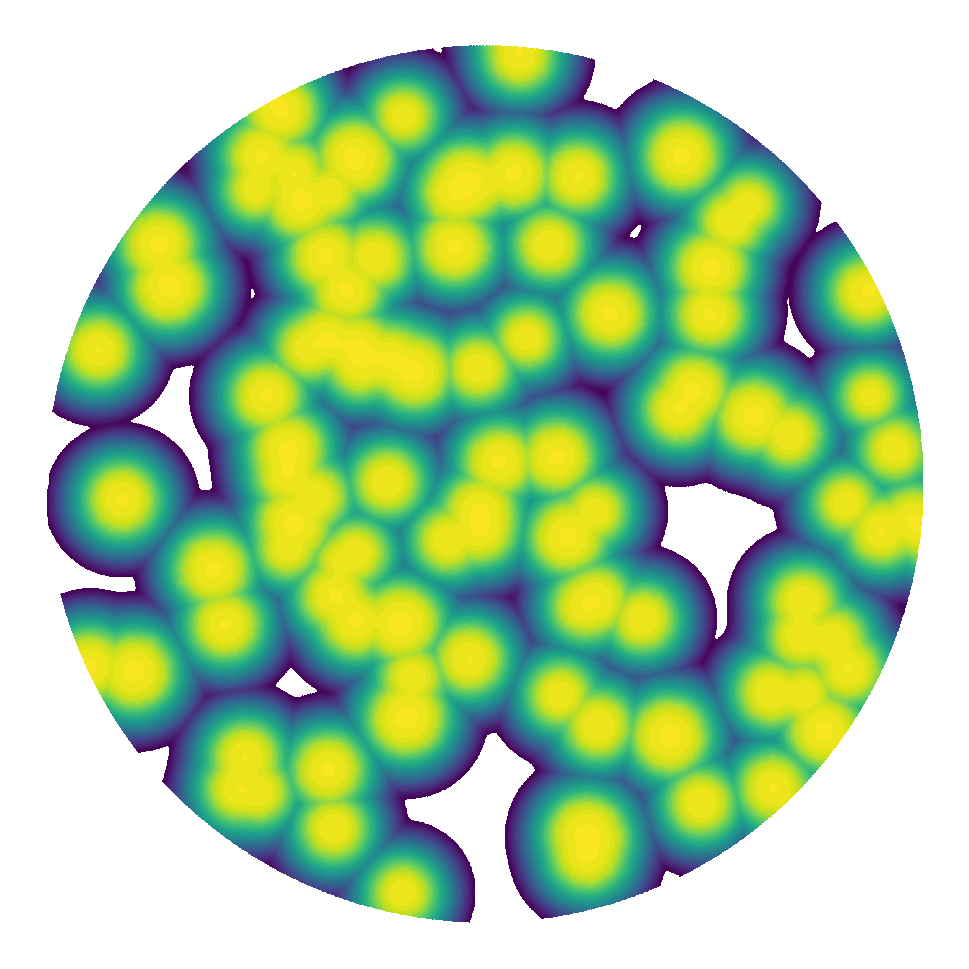
\includegraphics[width=0.48\textwidth]{Figures/Full-Dish-VirusPhotos/virus39.png}}

    \resizebox{0.48\textwidth}{!}{%
        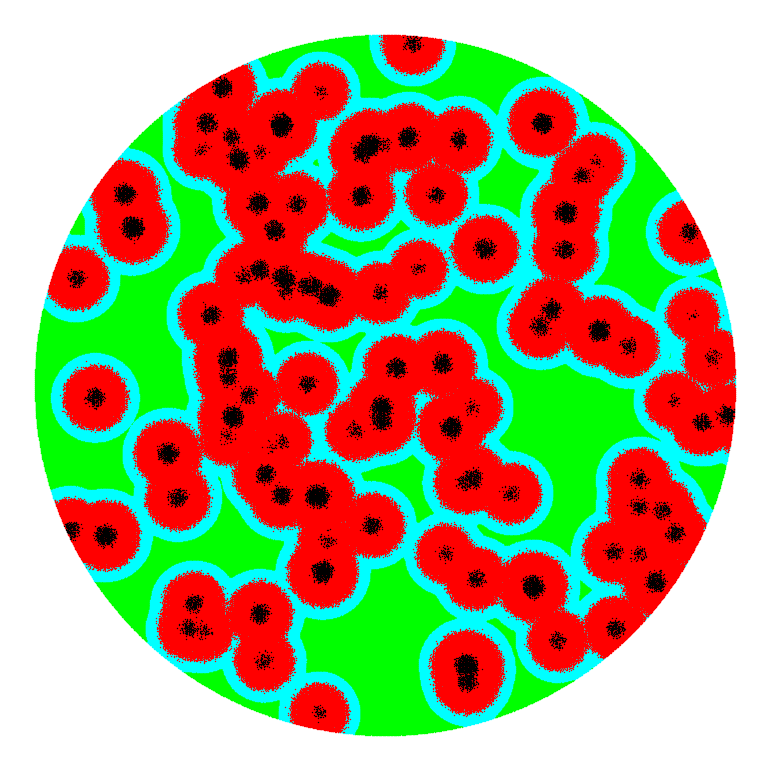
\includegraphics[width=0.48\textwidth]{Figures/Full-Dish-CellPhotos/cell49.png}
        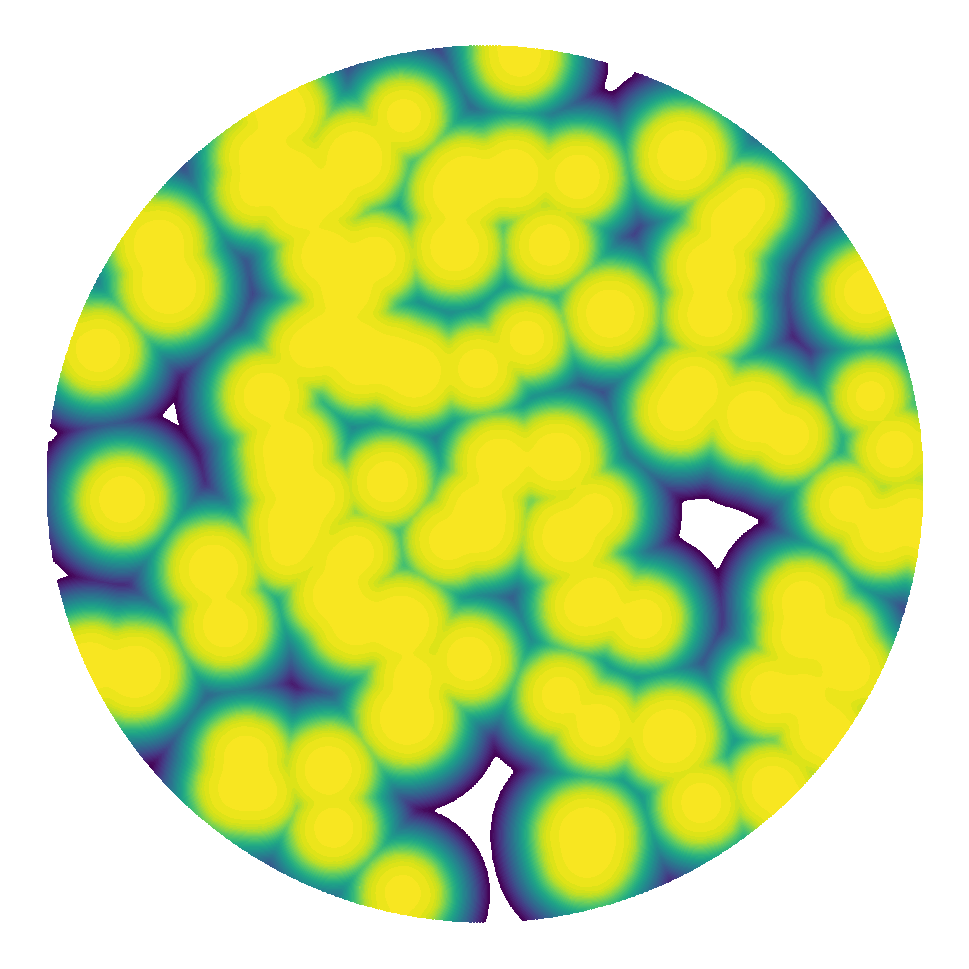
\includegraphics[width=0.48\textwidth]{Figures/Full-Dish-VirusPhotos/virus49.png}}

    \resizebox{0.48\textwidth}{!}{%
        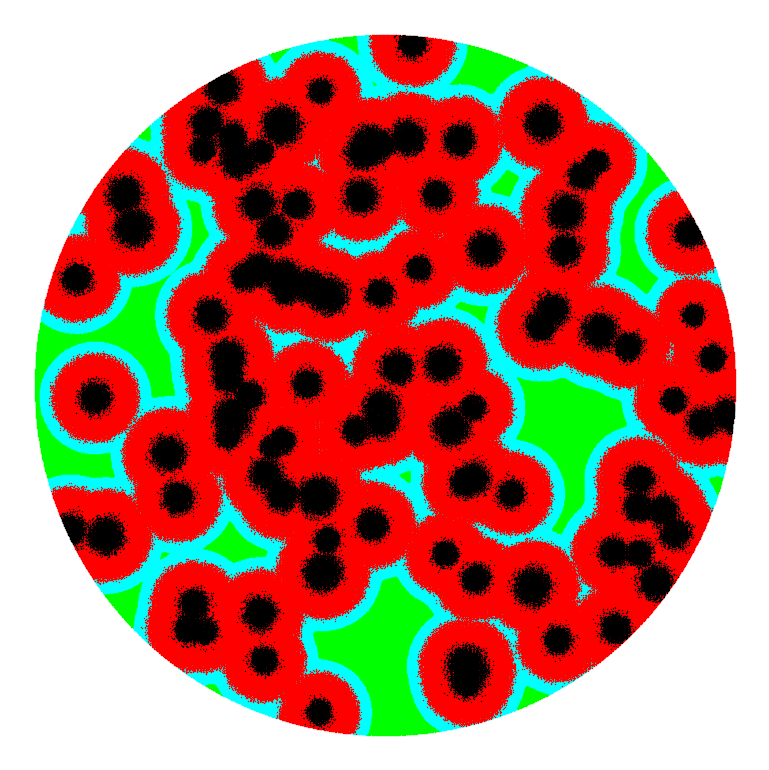
\includegraphics[width=0.48\textwidth]{Figures/Full-Dish-CellPhotos/cell59.png}
        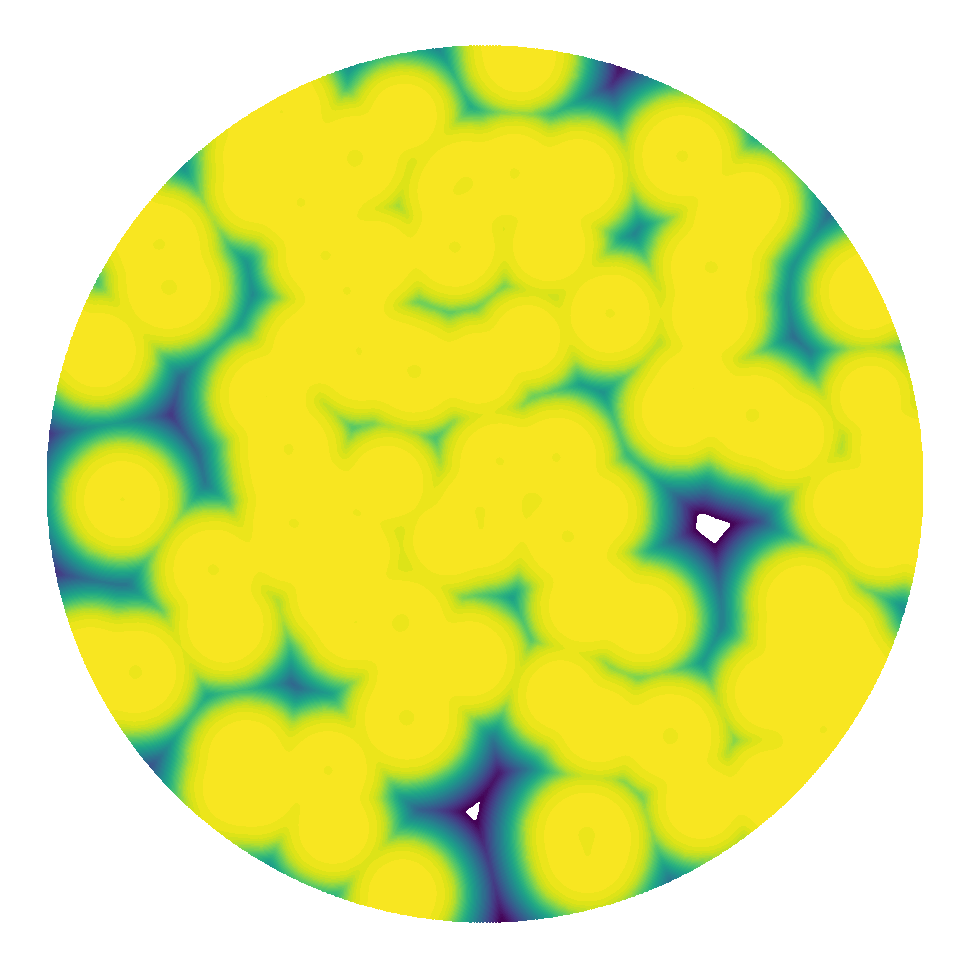
\includegraphics[width=0.48\textwidth]{Figures/Full-Dish-VirusPhotos/virus59.png}}

    \resizebox{0.48\textwidth}{!}{%
        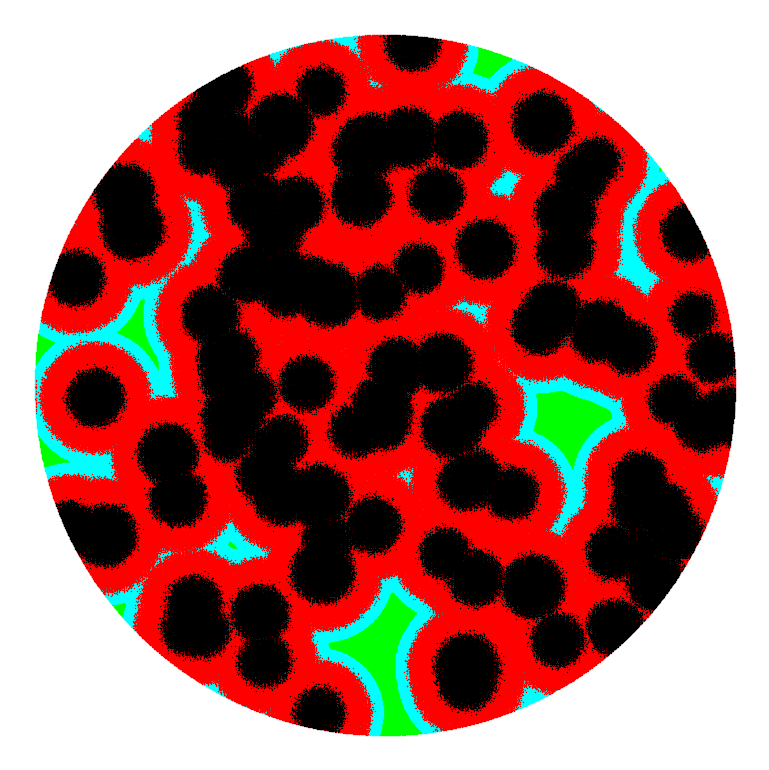
\includegraphics[width=0.48\textwidth]{Figures/Full-Dish-CellPhotos/cell69.png}
        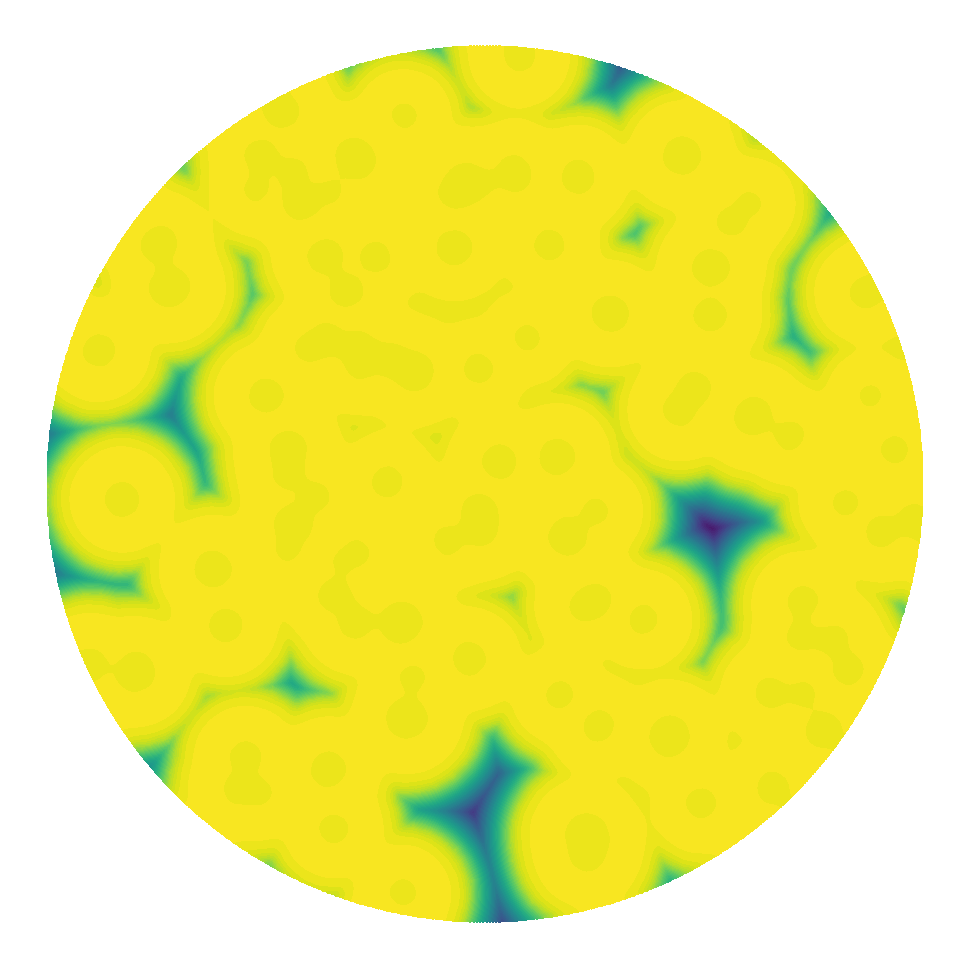
\includegraphics[width=0.48\textwidth]{Figures/Full-Dish-VirusPhotos/virus69.png}}

    \resizebox{0.48\textwidth}{!}{%
        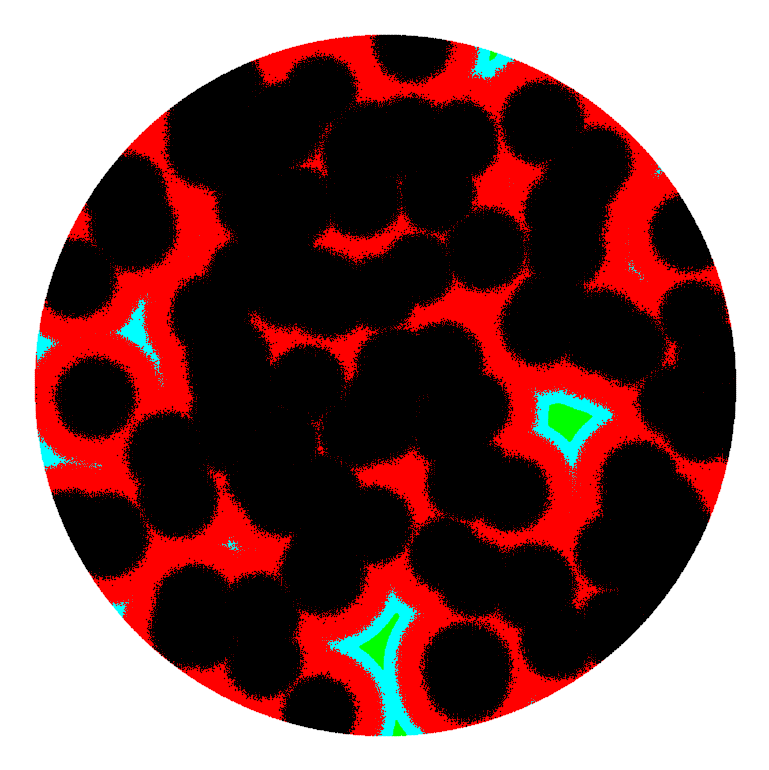
\includegraphics[width=0.48\textwidth]{Figures/Full-Dish-CellPhotos/cell79.png}
        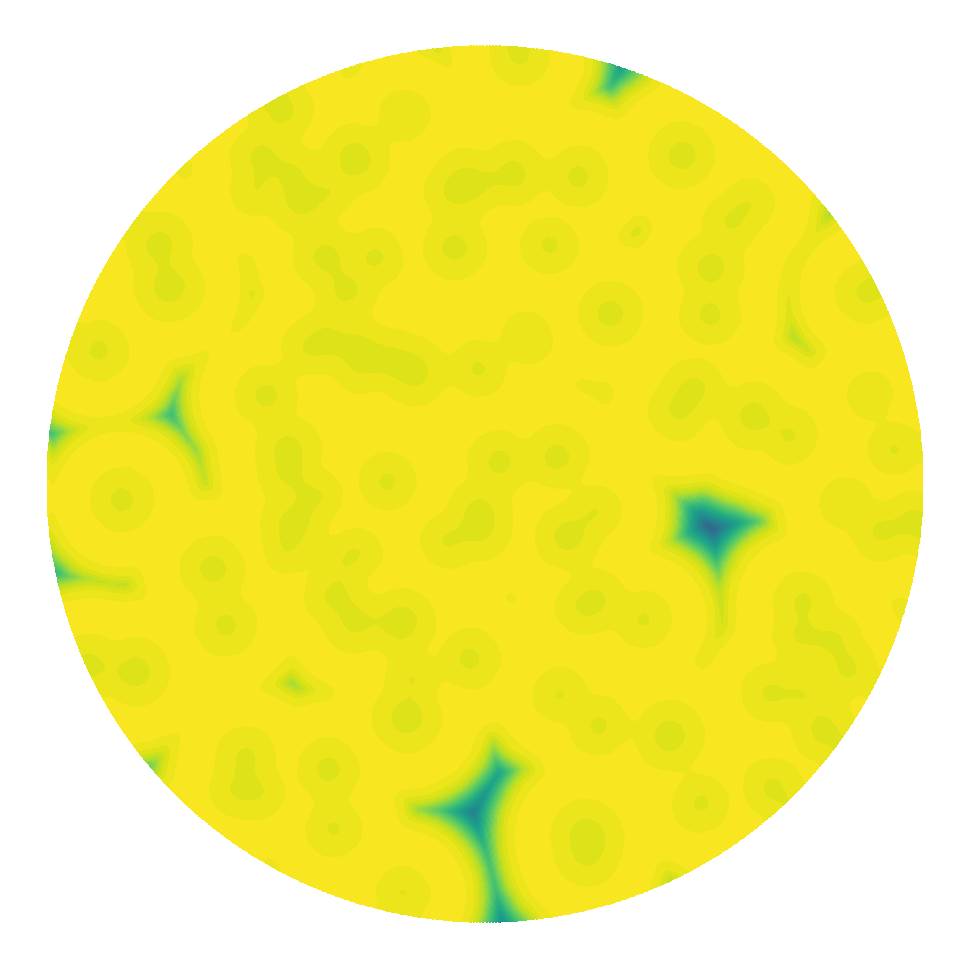
\includegraphics[width=0.48\textwidth]{Figures/Full-Dish-VirusPhotos/virus79.png}}

    \resizebox{0.48\textwidth}{!}{% 
        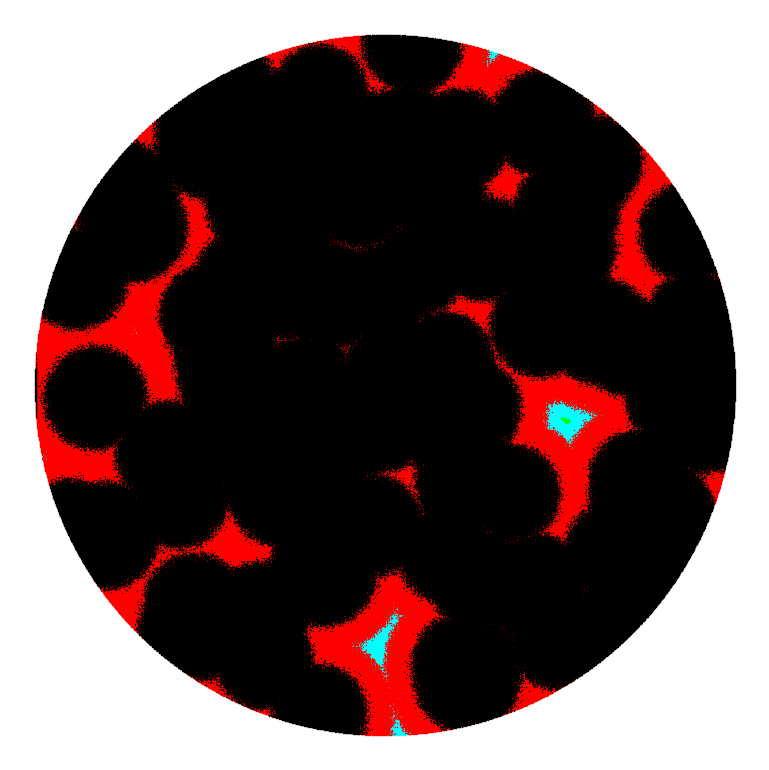
\includegraphics[width=0.48\textwidth]{Figures/Full-Dish-CellPhotos/cell89.png}
        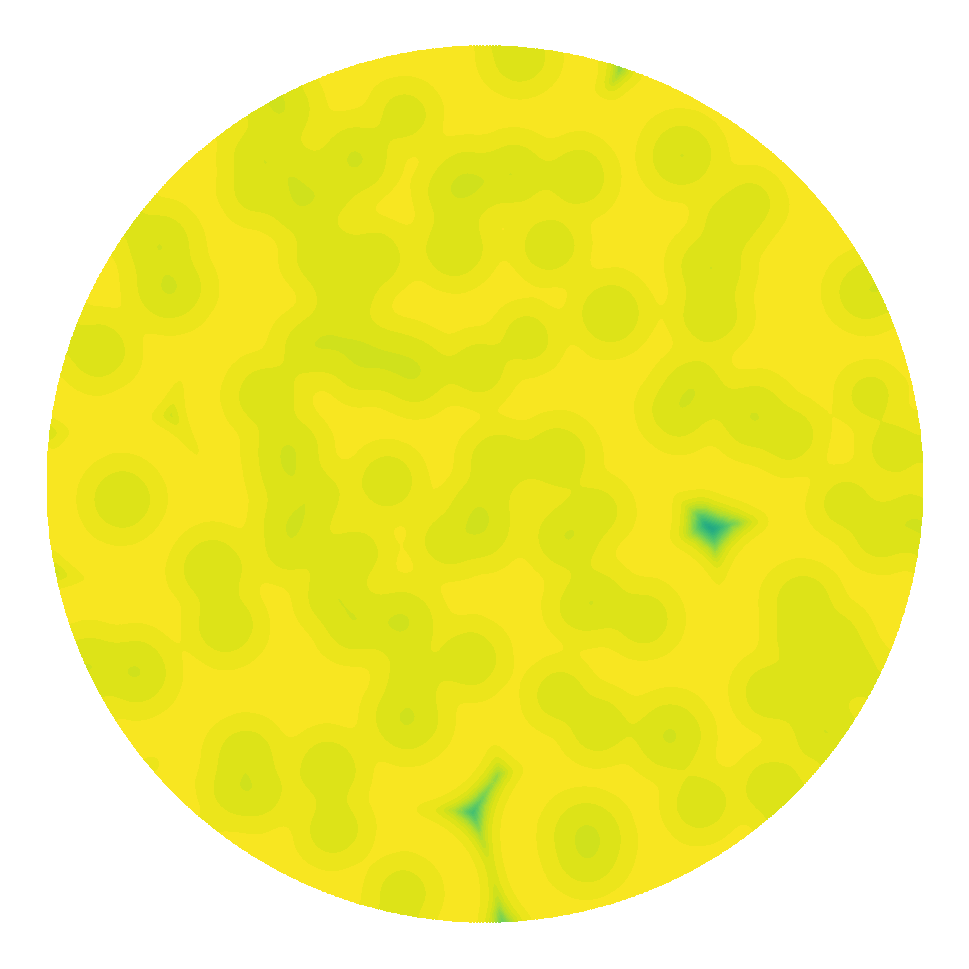
\includegraphics[width=0.48\textwidth]{Figures/Full-Dish-VirusPhotos/virus89.png}}

    \resizebox{0.48\textwidth}{!}{%
        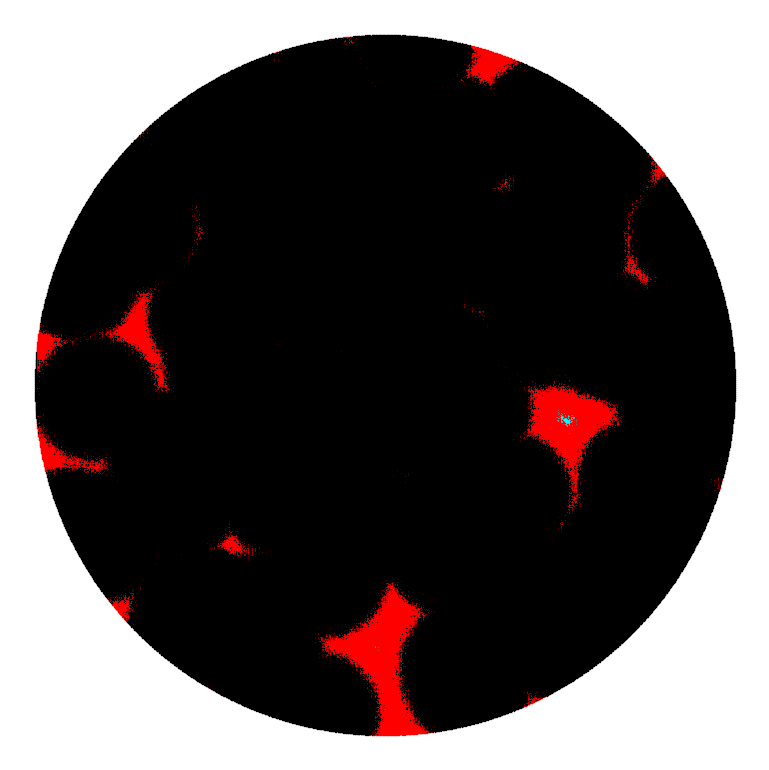
\includegraphics[width=0.48\textwidth]{Figures/Full-Dish-CellPhotos/cell99.png}
        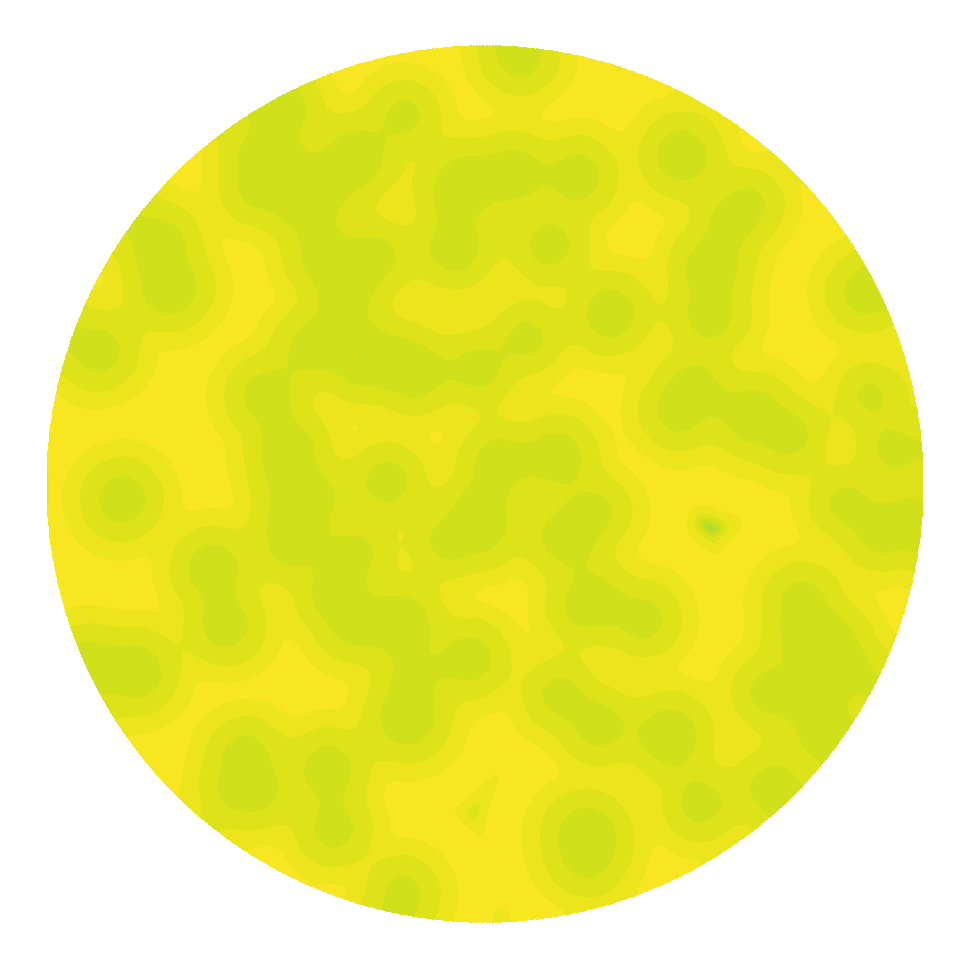
\includegraphics[width=0.48\textwidth]{Figures/Full-Dish-VirusPhotos/virus99.png}}

    \resizebox{0.48\textwidth}{!}{%
        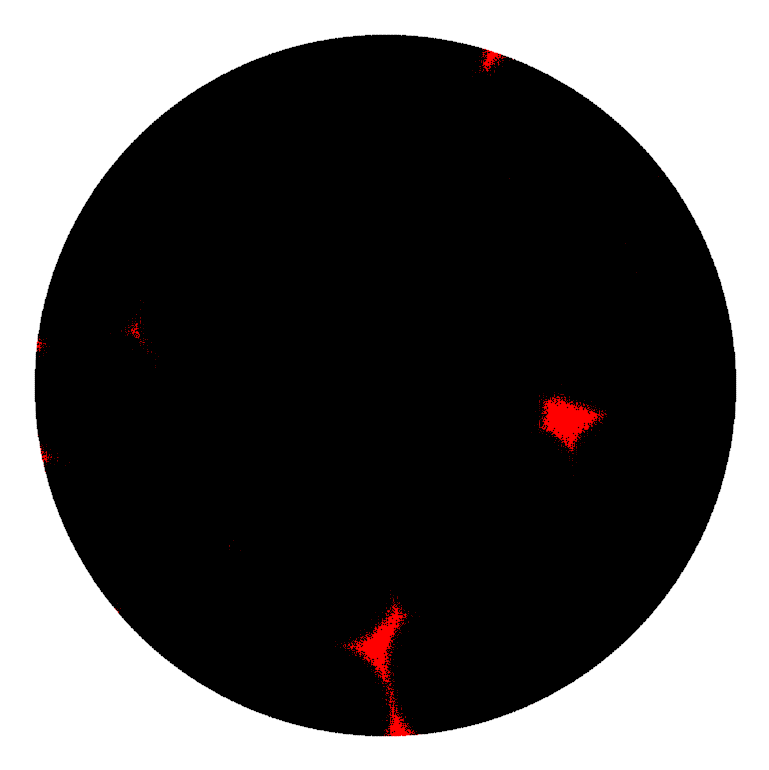
\includegraphics[width=0.48\textwidth]{Figures/Full-Dish-CellPhotos/cell109.png}
        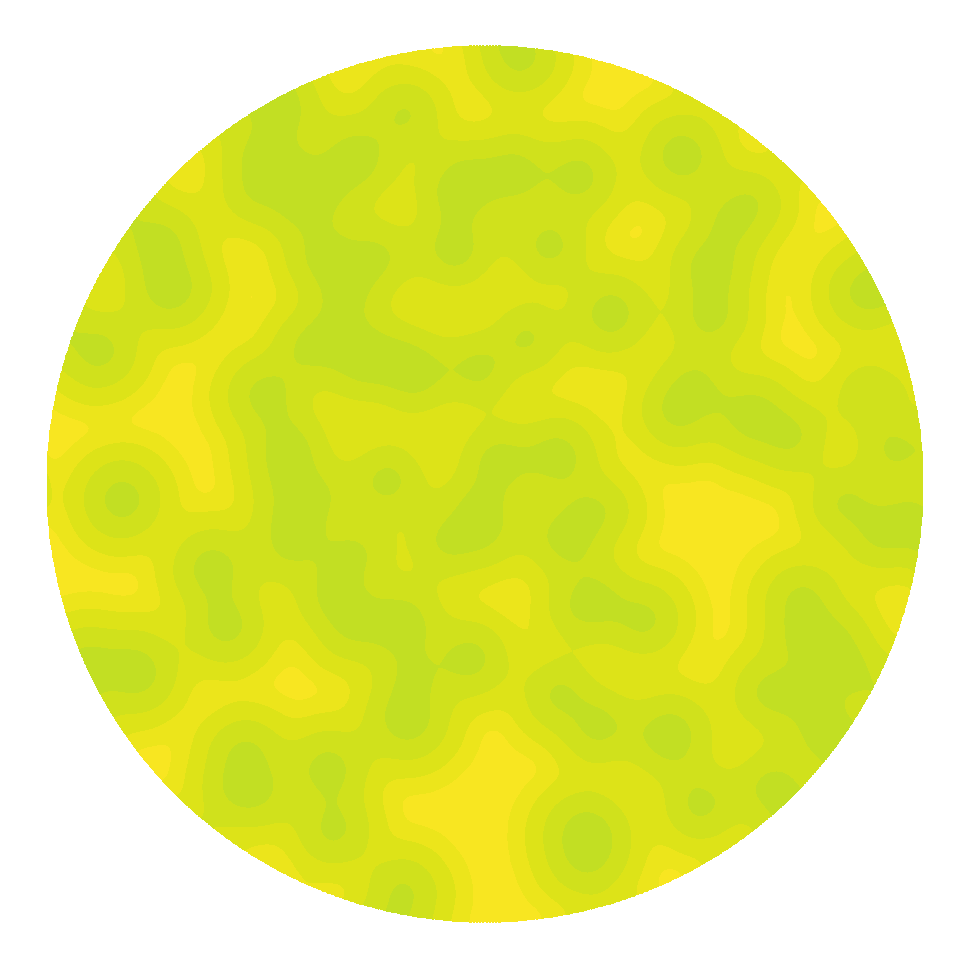
\includegraphics[width=0.48\textwidth]{Figures/Full-Dish-VirusPhotos/virus109.png}}

    \resizebox{0.48\textwidth}{!}{%
        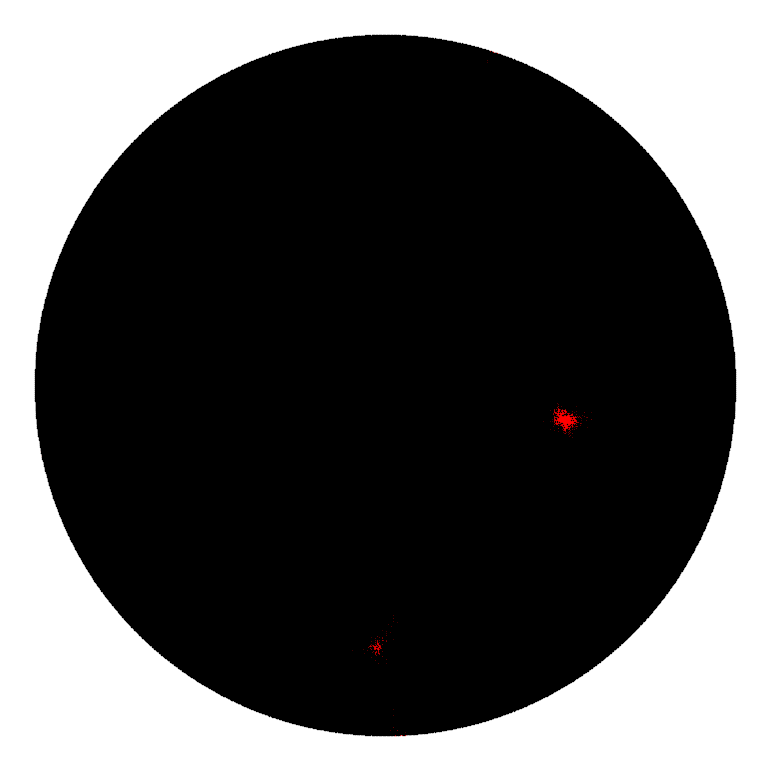
\includegraphics[width=0.48\textwidth]{Figures/Full-Dish-CellPhotos/cell119.png}
        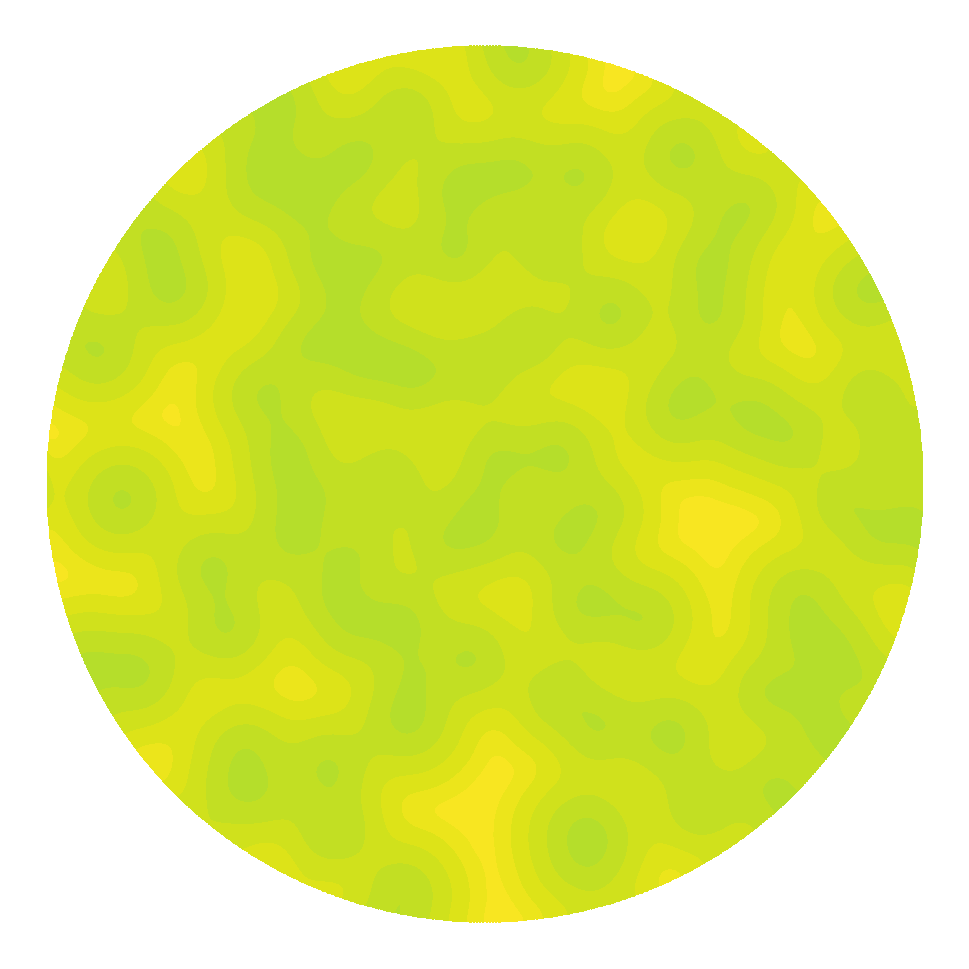
\includegraphics[width=0.48\textwidth]{Figures/Full-Dish-VirusPhotos/virus119.png}}

\end{multicols}
\end{minipage}
\caption{The dish at hours 5 through 60 in 5 hour increments. On the left are cells in the different stages of infection; the stages are represented by healthy cells colored green, eclipse cells colored cyan, infected cells colored red, and dead cells colored black. On the right are images of the virions that are diffusing over the cells; areas of higher concentration are represented by yellow and areas of lower concentration are represented by purple. \label{fig_FullDish_cellandvirus}}
\end{figure}

For a closer look at the plaques, figure \ref{fig_ZoominDish} is a zoomed in view of the infection at hours 6.5, 11.5, and 16.5. The cells are shown on the left, with the same color scheme used in figure \ref{fig_FullDish_cellandvirus}, and the corresponding virus distribution is shown on the right. Here the heterogeneous growth of the plaque can clearly be see; it is not simply a radially symmetric change of cells from eclipse to infectious. 

\begin{figure}
\centering
\begin{minipage}{0.66\linewidth}
\centering
    \resizebox{\textwidth}{!}{%
        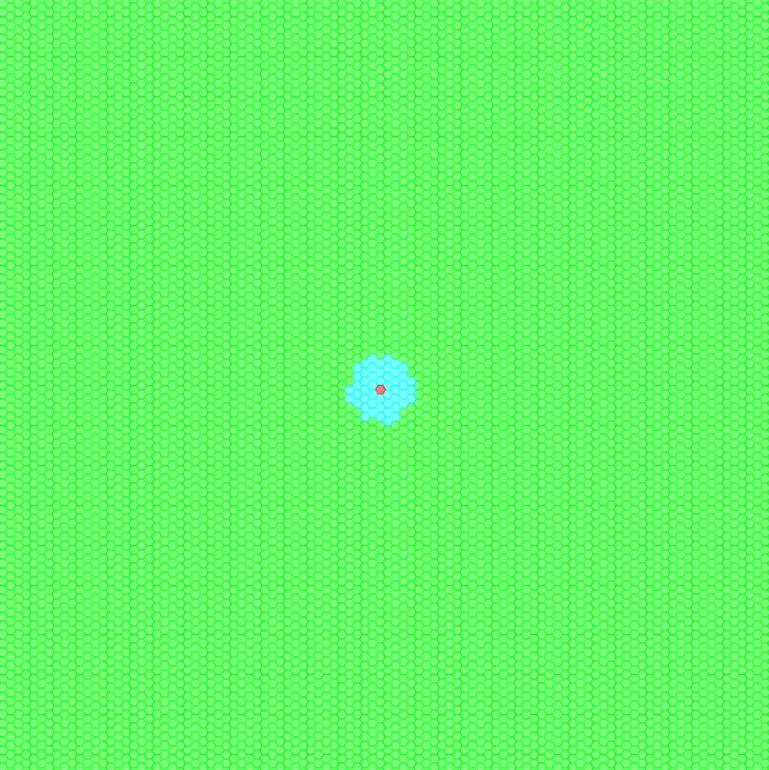
\includegraphics[width=0.48\textwidth]{Figures/Zoomed-In-CellPhotos/cell12.png}
        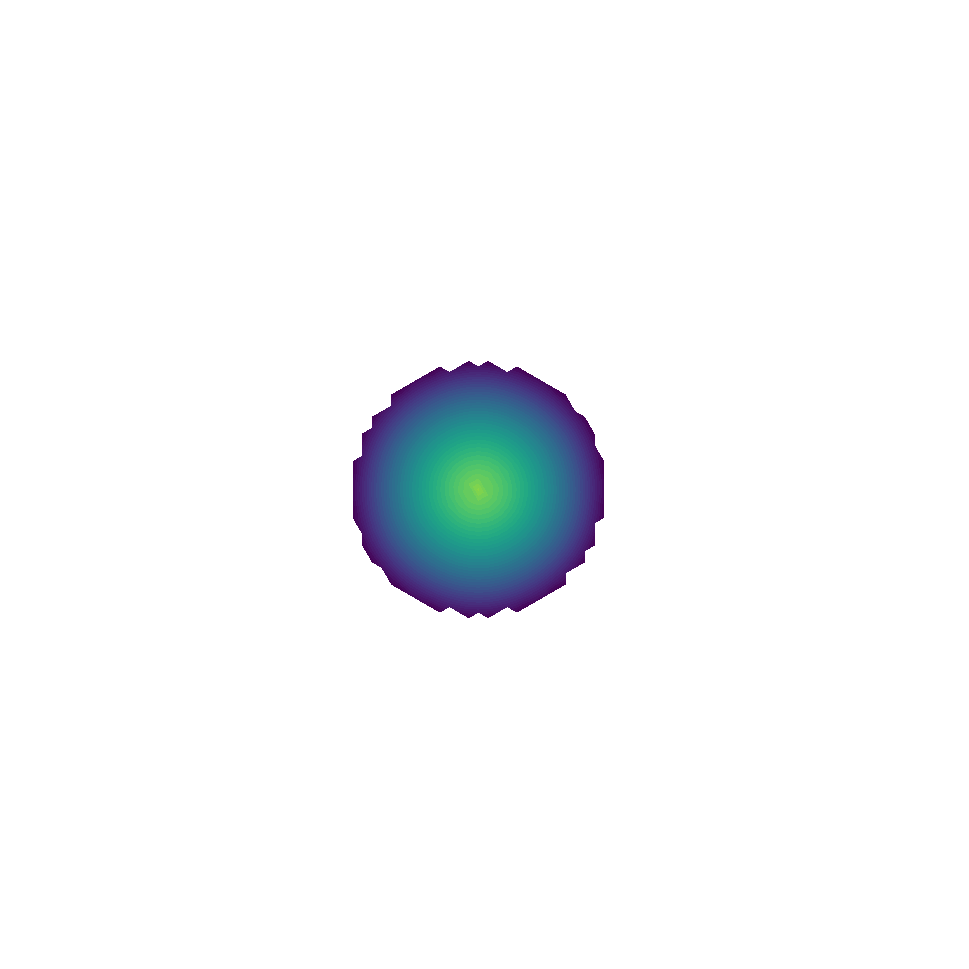
\includegraphics[width=0.48\textwidth]{Figures/Zoomed-In-VirusPhotos/virus12.png}}

    \vspace{0.25em}
    \resizebox{\textwidth}{!}{%
        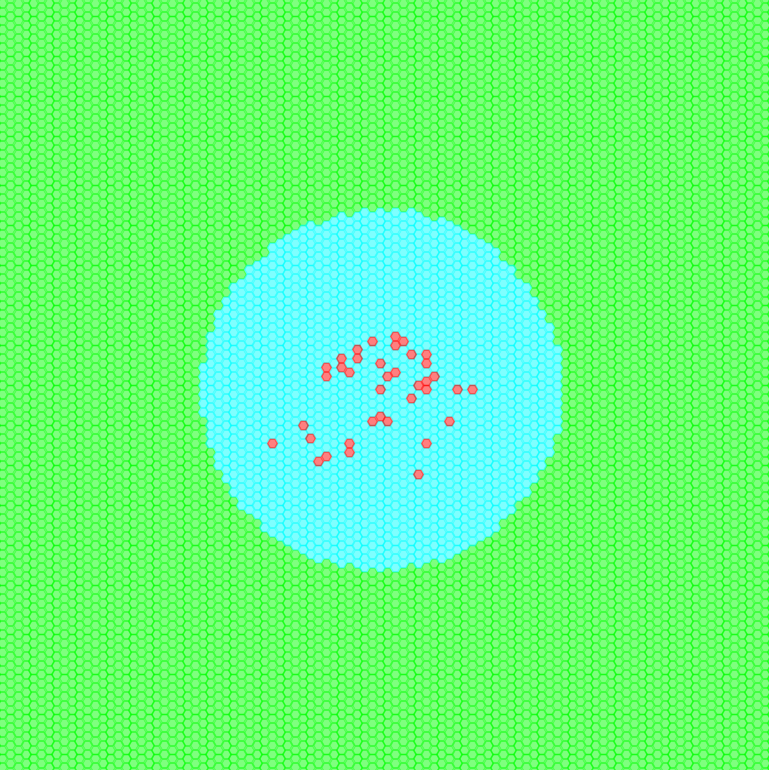
\includegraphics[width=0.48\textwidth]{Figures/Zoomed-In-CellPhotos/cell22.png}
        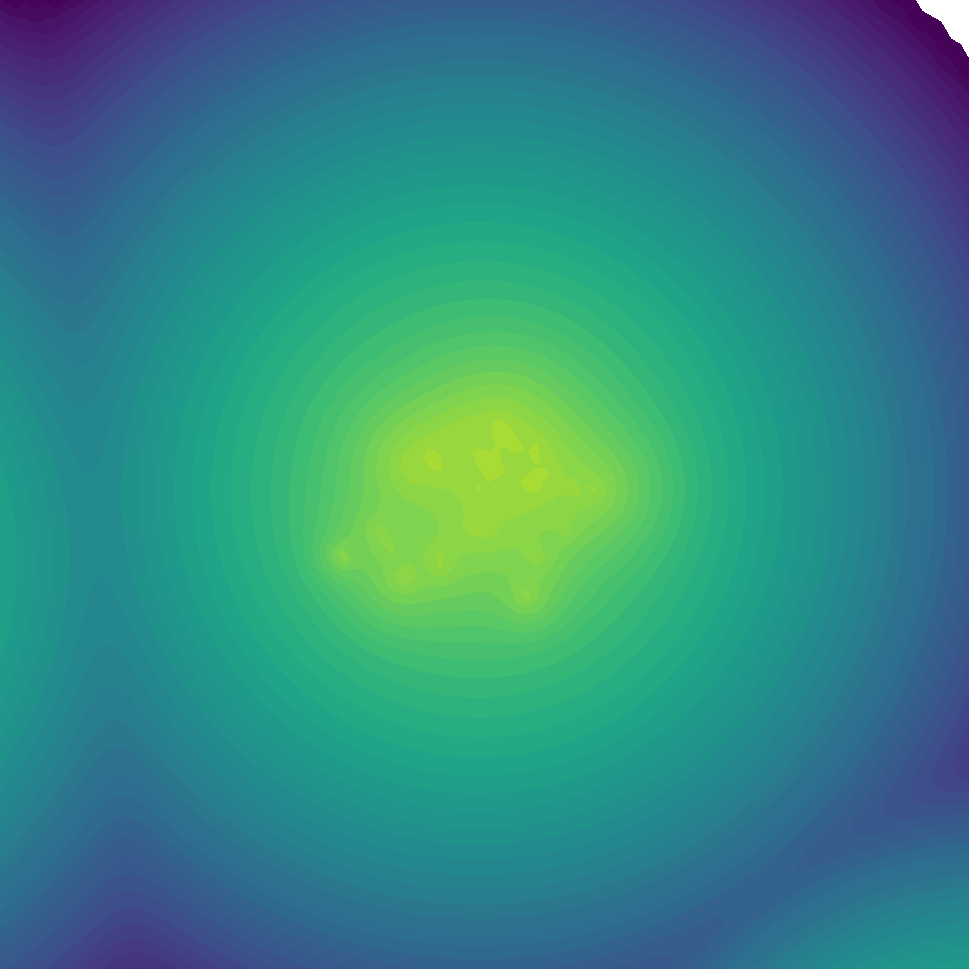
\includegraphics[width=0.48\textwidth]{Figures/Zoomed-In-VirusPhotos/virus22.png}}

    \vspace{0.25em}
    \resizebox{\textwidth}{!}{%
        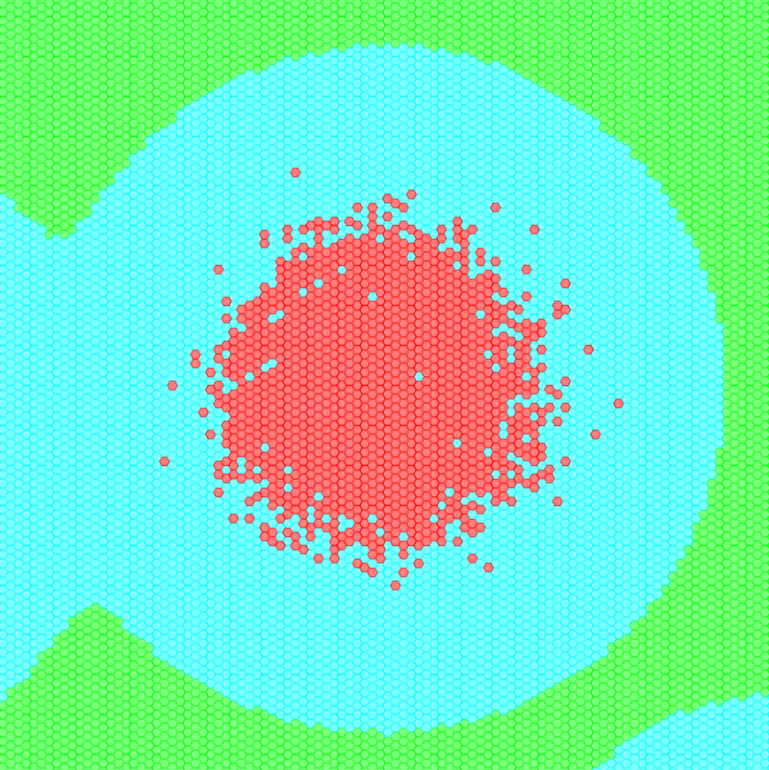
\includegraphics[width=0.48\textwidth]{Figures/Zoomed-In-CellPhotos/cell32.png}
        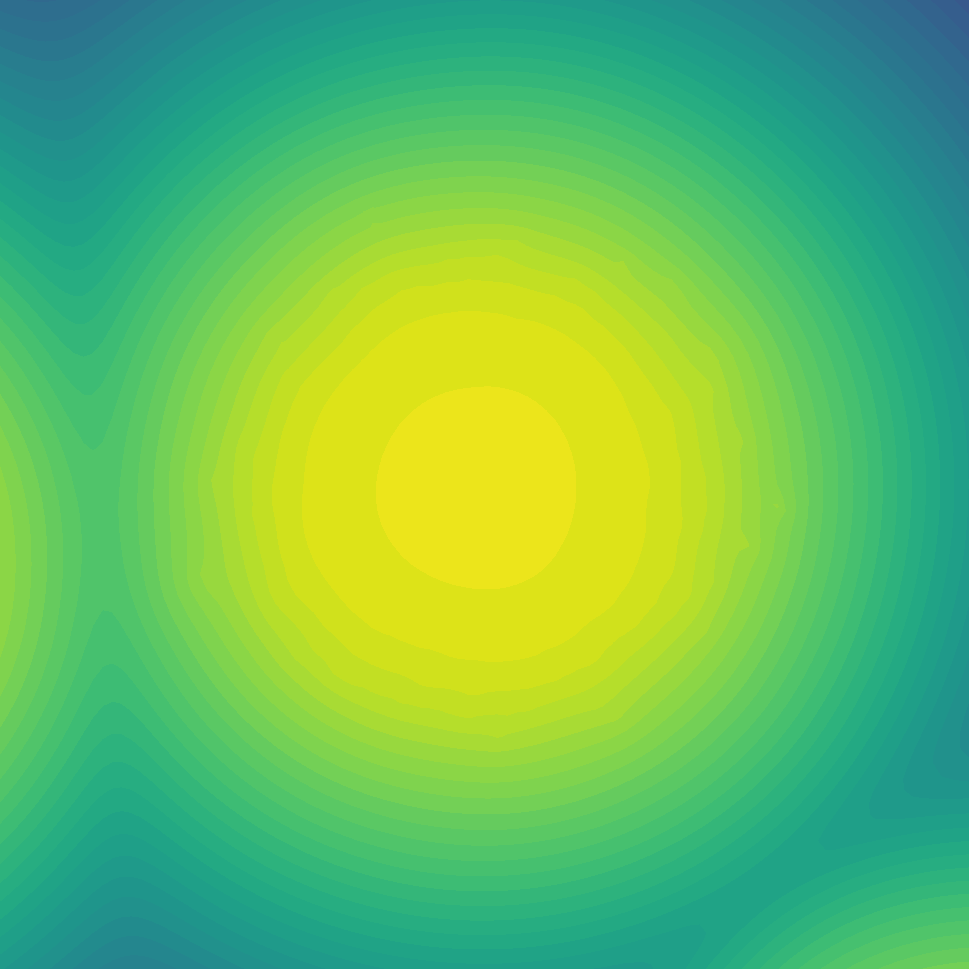
\includegraphics[width=0.48\textwidth]{Figures/Zoomed-In-VirusPhotos/virus32.png}}
\end{minipage}
\caption{A zoomed in section of the dish looking at the plaque formed by a single infected cell during a viral infection at hours 6.5, 11.5, and 16.5. On the left are cells in the different stages of infection; the stages are represented by healthy cells colored green, eclipse cells colored cyan, infected cells colored red, and dead cells colored black. On the right are the many virus that are diffusing over the cells; areas of higher concentration are represented by yellow and areas of lower concentration are represented by purple. \label{fig_ZoominDish}}
\end{figure}

As a visual check, the simulated plaque assays are compared to actual plaque assays. The left of figure \ref{fig_Plaques} is a petri dish from a plaque assay that infected MDCK cells with influenza virus A/Memphis/14/96-M (H1N1). The virus was placed in the dish and then after one hour a solution of Avicel RC-581 was injected onto the cells. The Avicel RC-581 allows for plaques to form by hindering the flow of virus through the liquid medium in the dish. When the experiment was done, the assays were stained with an immuno-stain that stains the infected cells red. The right of figure \ref{fig_Plaques} shows the simulated assay of $10^{6}$ cells, where again the same color scheme as figure \ref{fig_FullDish_cellandvirus} is used; the healthy cells are colored green, eclipse cells are colored cyan, infected cells are colored red, and dead cells are colored black. The plaques appear to be similar between the actual and simulated assays.

\begin{figure}[h]
    \centering
    \resizebox{\textwidth}{!}{%
        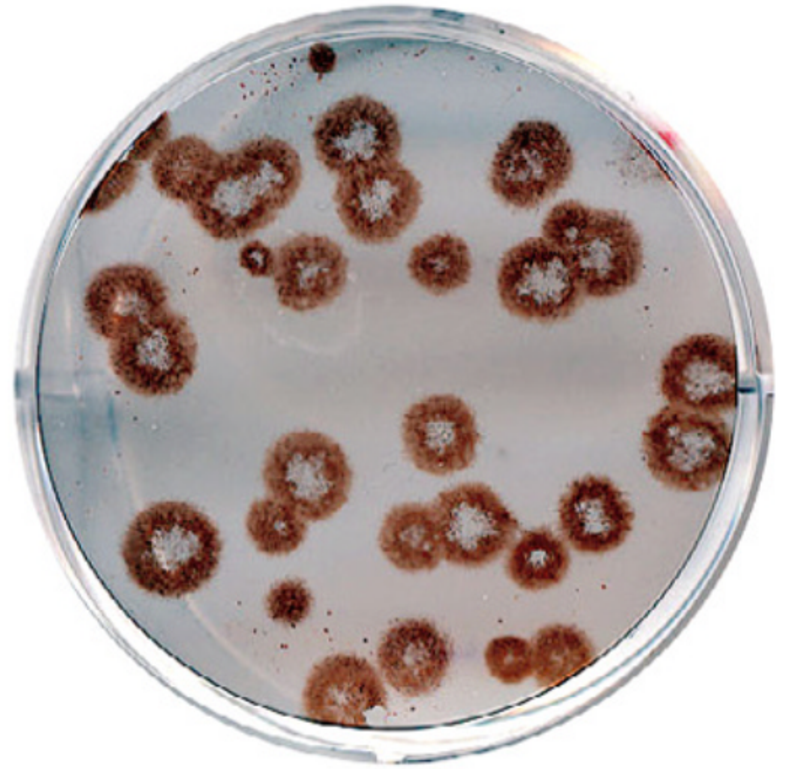
\includegraphics[width=0.48\textwidth]{Figures/plaques.pdf}
        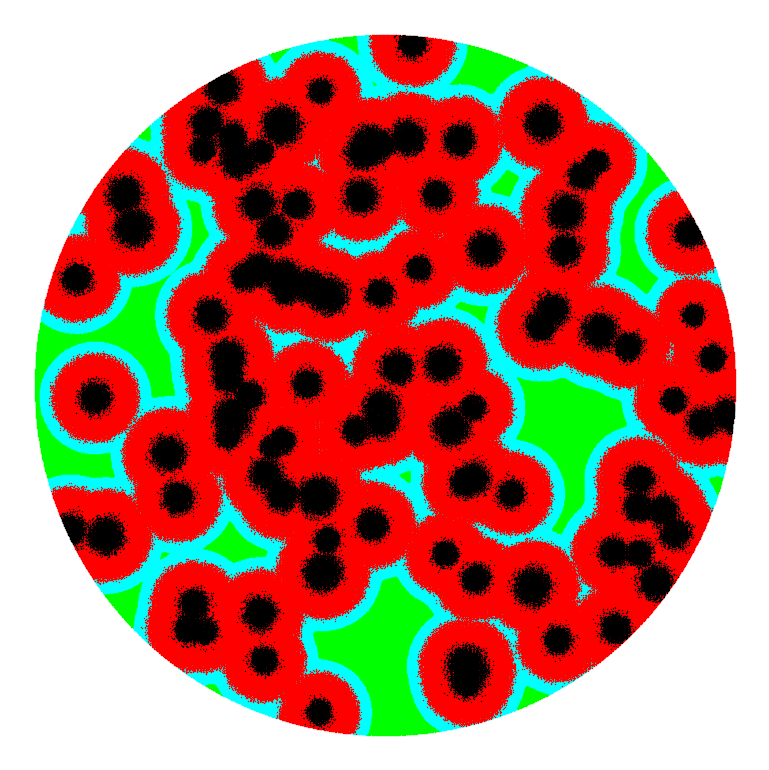
\includegraphics[width=0.48\textwidth]{Figures/Full-Dish-CellPhotos/cell59.png}}

\caption{(Left) Plaque assay that infected MDCK cells with influenza virus A/Memphis/14/96-M (H1N1). (Right) Simulated plaque assay of $10^{6}$ cells, where the green are the healthy cells, cyan are the eclipse cells, red are the infected cells, and black are the dead cells. \label{fig_Plaques}}
\end{figure}

\section{Implementation on GPUs}

Ten viral infections of five different numbers of cells were simulated, with codes that utilize three different programming languages: Python, C, and CUDA. The amount of computation time needed to simulate one hour of the infection, on a desktop computer, is shown in figure \ref{fig:SpeedComparison}. The computer was built with an Intel Xeon E-2144G central processing unit (CPU), 16 gigabytes of random access memory (RAM), and P4000 Nvidia Graphics card. The compute times for the three codes increase as the number of cells in the simulations increases, but the speed increase of switching from Python, the programming language commonly used in physics, to code using CUDA for implementation on GPUs is 6954 times faster.
\begin{figure}
    \centering
    \resizebox{0.6\textwidth}{!}{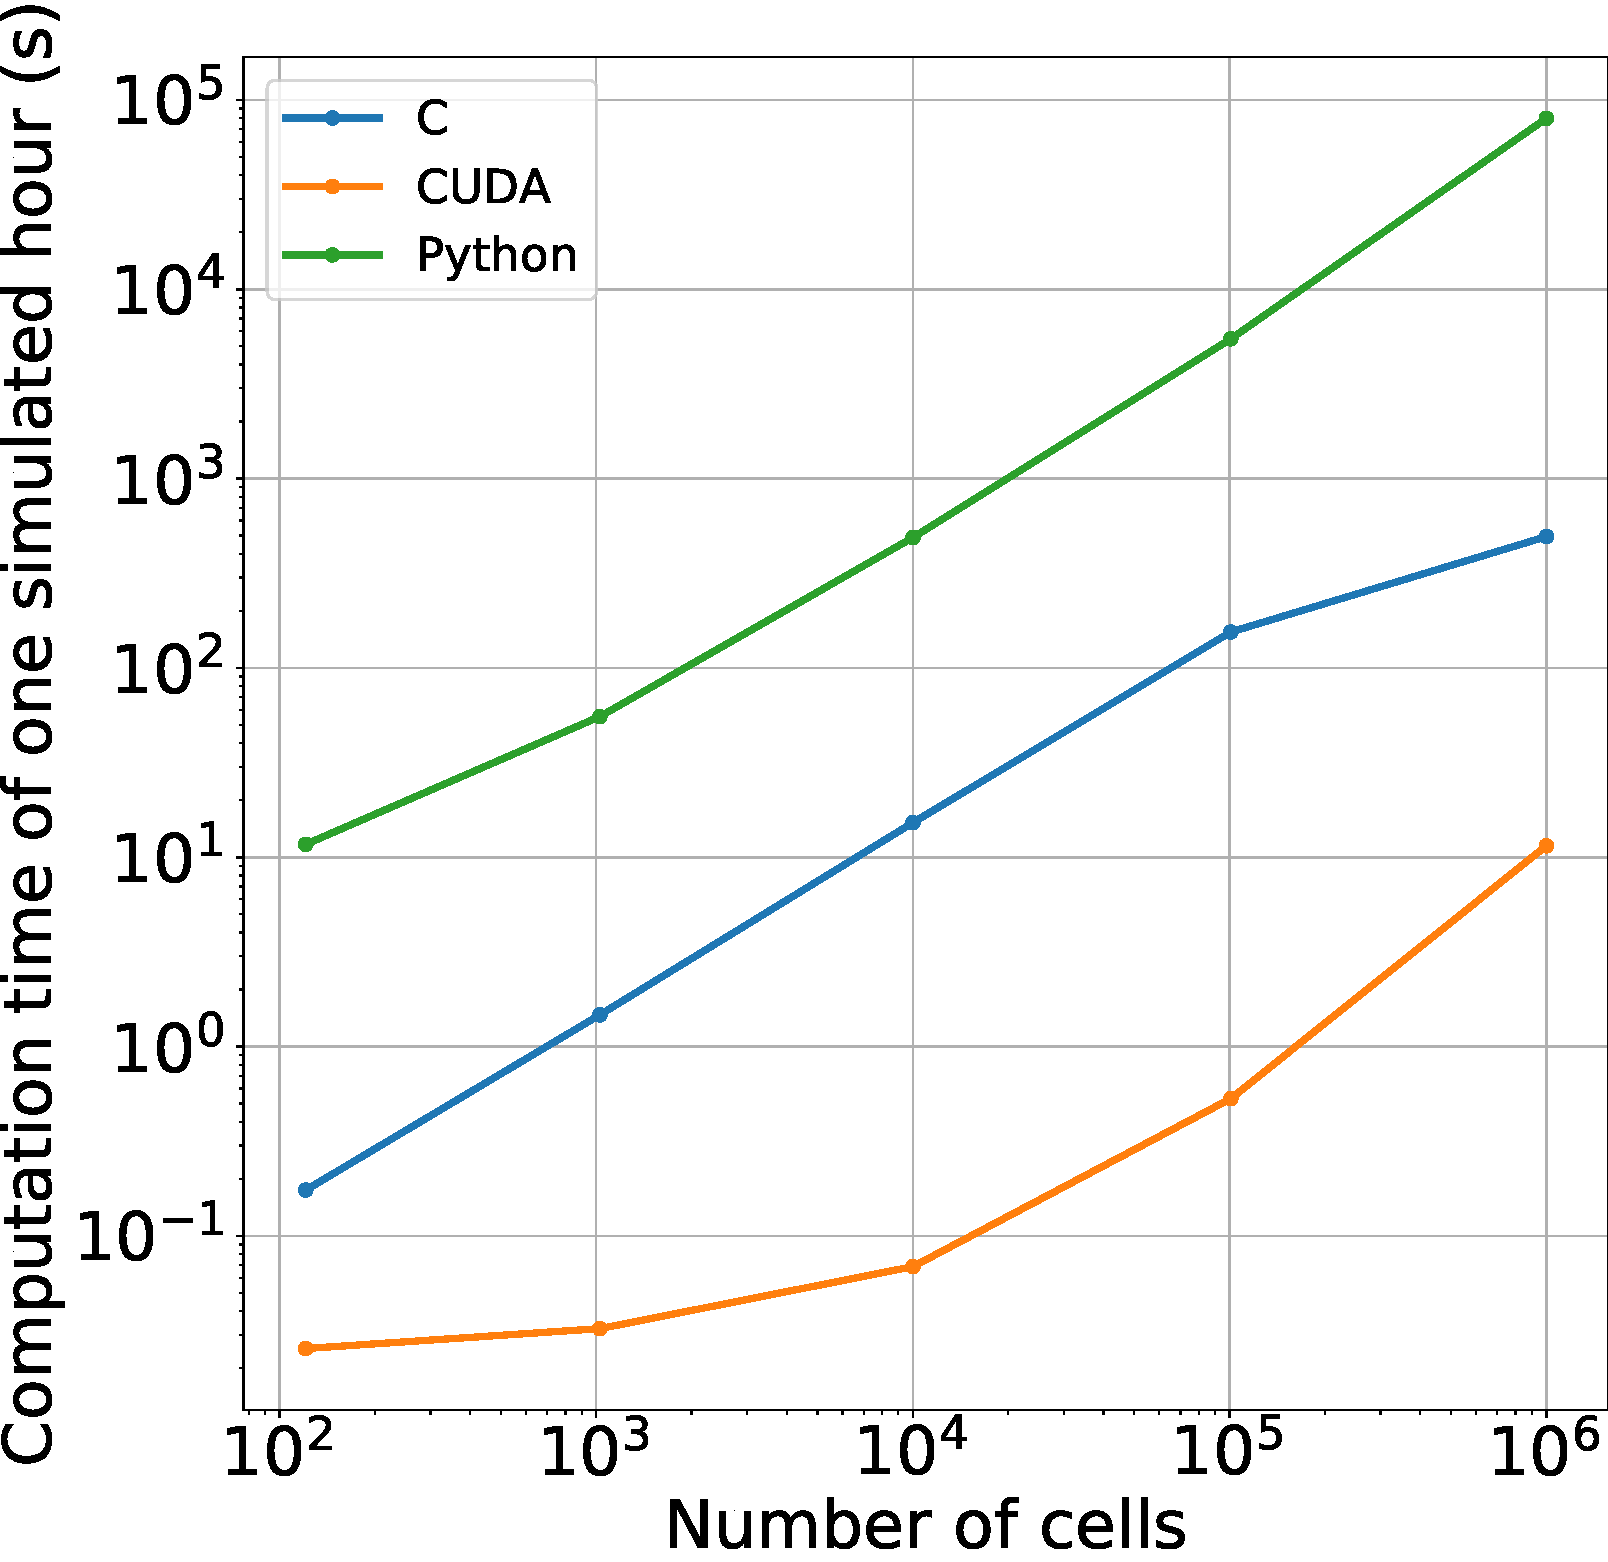
\includegraphics{Figures/loglogspeed.pdf}}
\caption{With more than a million cells, CUDA is 6954 times faster then the Python code and 43 time faster than the C code. \label{fig:SpeedComparison}}
\end{figure}

%\clearpage
\section{Convergence Testing}

Three scenarios were examined when testing the convergence of the model: an infection initiated with $10013$ cells in the eclipse phase (Initial Cell); an infection initiated with $10^{12}$ virions (Initial Virus); and a scenario with no infection, but $10^{12}$ virions (Only Virus), examining viral spread and decay only. Simulations in each of the scenarios used the influenza parameters from table \ref{tab_params}. Figure \ref{fig:ViralTiterCurves} shows the simulations of the three scenarios, where the time step was varied to test the convergence of the model in time. A time step of 0.005 hr, about 5.78 times smaller than the conditional relationship from section \ref{methods_convergance}, was chosen and a range around it was made by dividing or multiplying by 2 repeatedly. This formed an array of seven time step values, 0.000625, 0.00128, 0.0025, 0.005, 0.01, 0.02, and 0.04 hr. For each time step, the median curve of ten viral titer curves is shown. In figure \ref{fig:ViralTiterCurves}, from left to right, curves of a viral infection initiated with infected cells; curves of a viral infection initiated with virus; and curves of virus without underlying cell infection. For all time steps, except $0.04$ hr, the curves are hard to distinguish from one another and follow the same trend for each scenario. 

\begin{figure}
    \centering
    \parbox{\textwidth}{
    \fbox{\parbox{\textwidth}{\vspace{-1em}
    \begin{multicols}{3}
        \centering

        Initial Cell

        Initial Virus

        Only Virus
    \end{multicols}
    \vspace{-1em}}}

    \vspace{0.5em}
    \centering
        \resizebox{\textwidth}{!}{%
        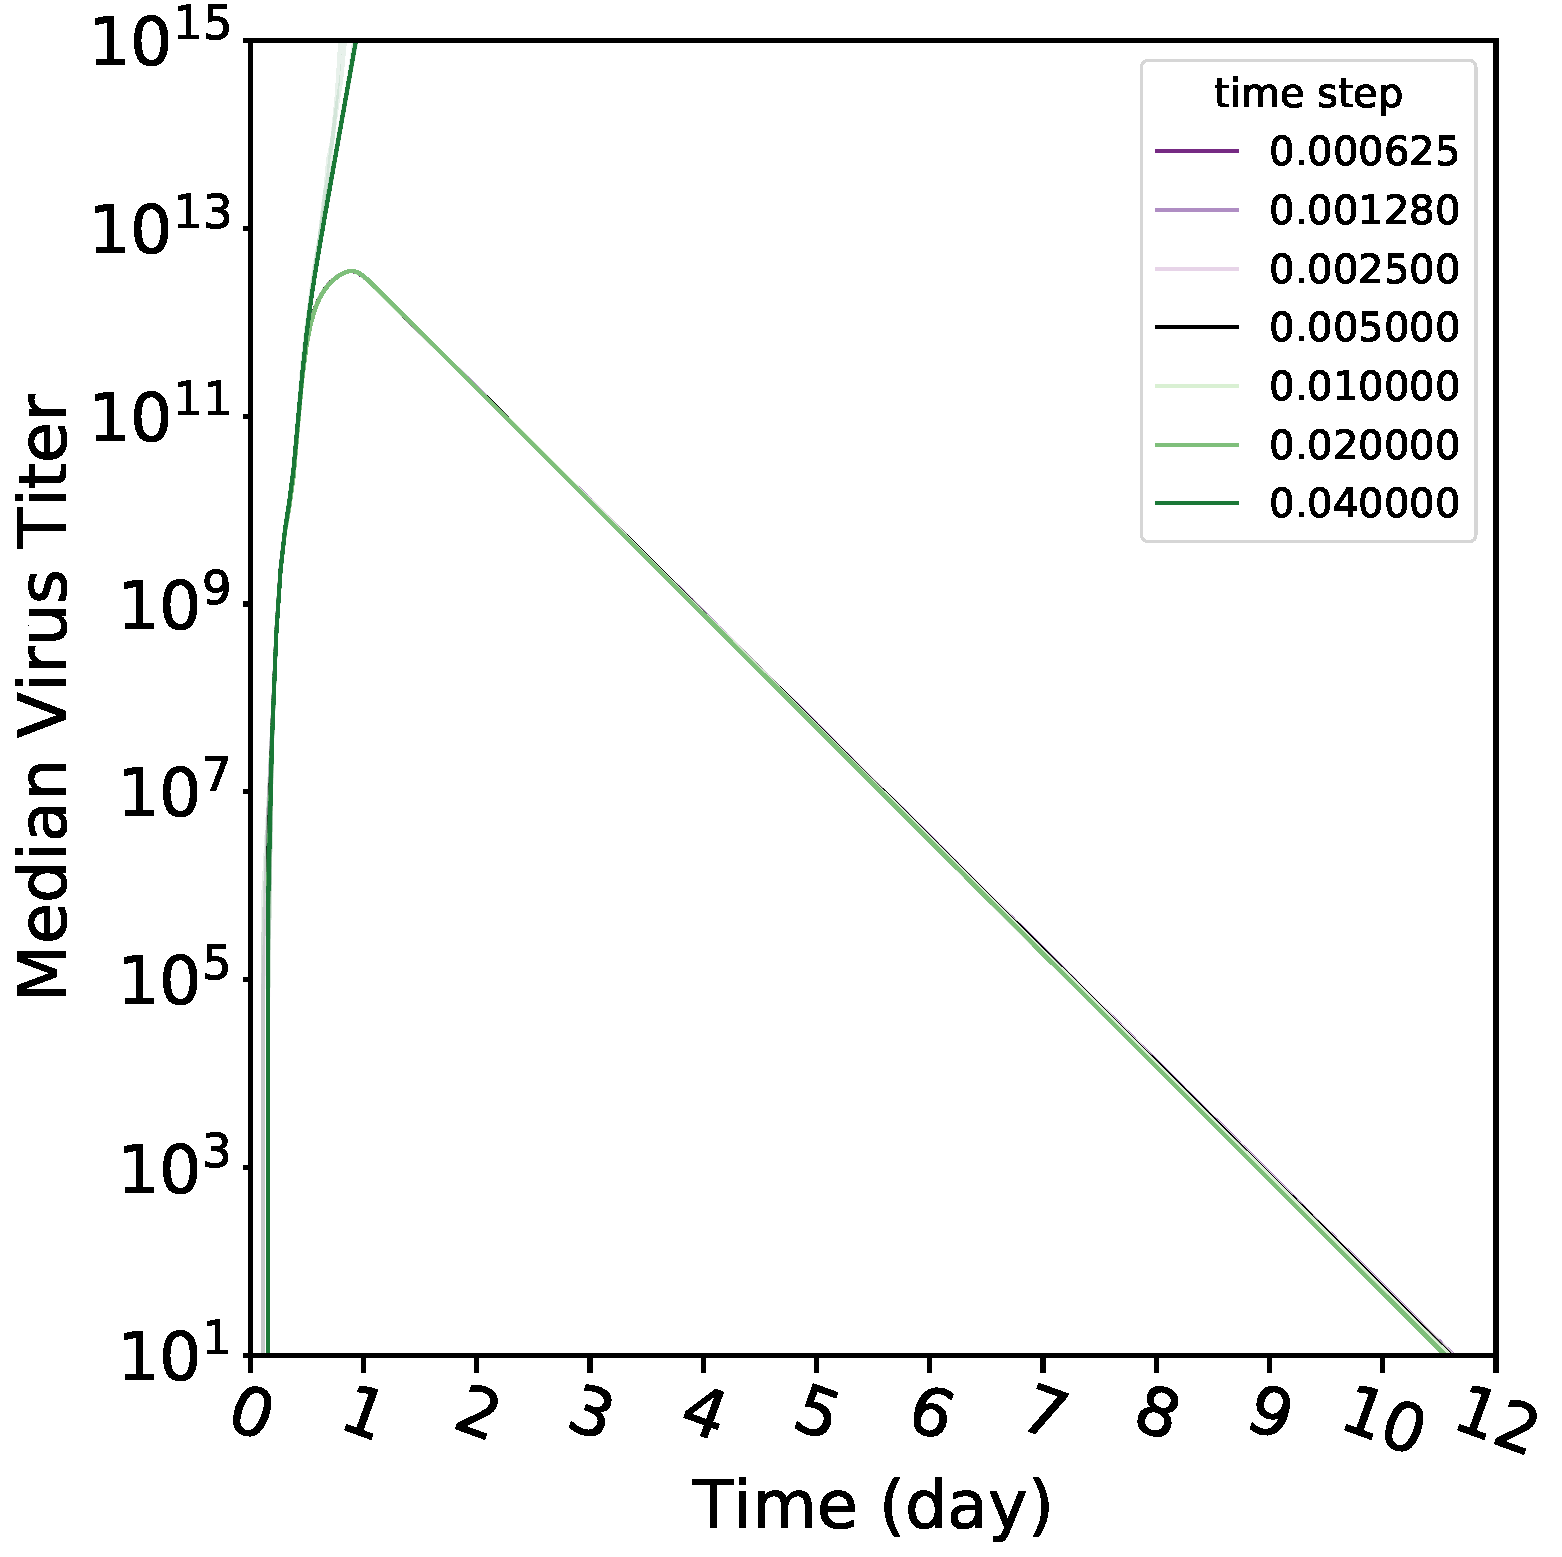
\includegraphics[width=0.33\linewidth]{Figures/Cellfree-InitialCell-AllOnOne_Median_VirusVsTime.pdf}
        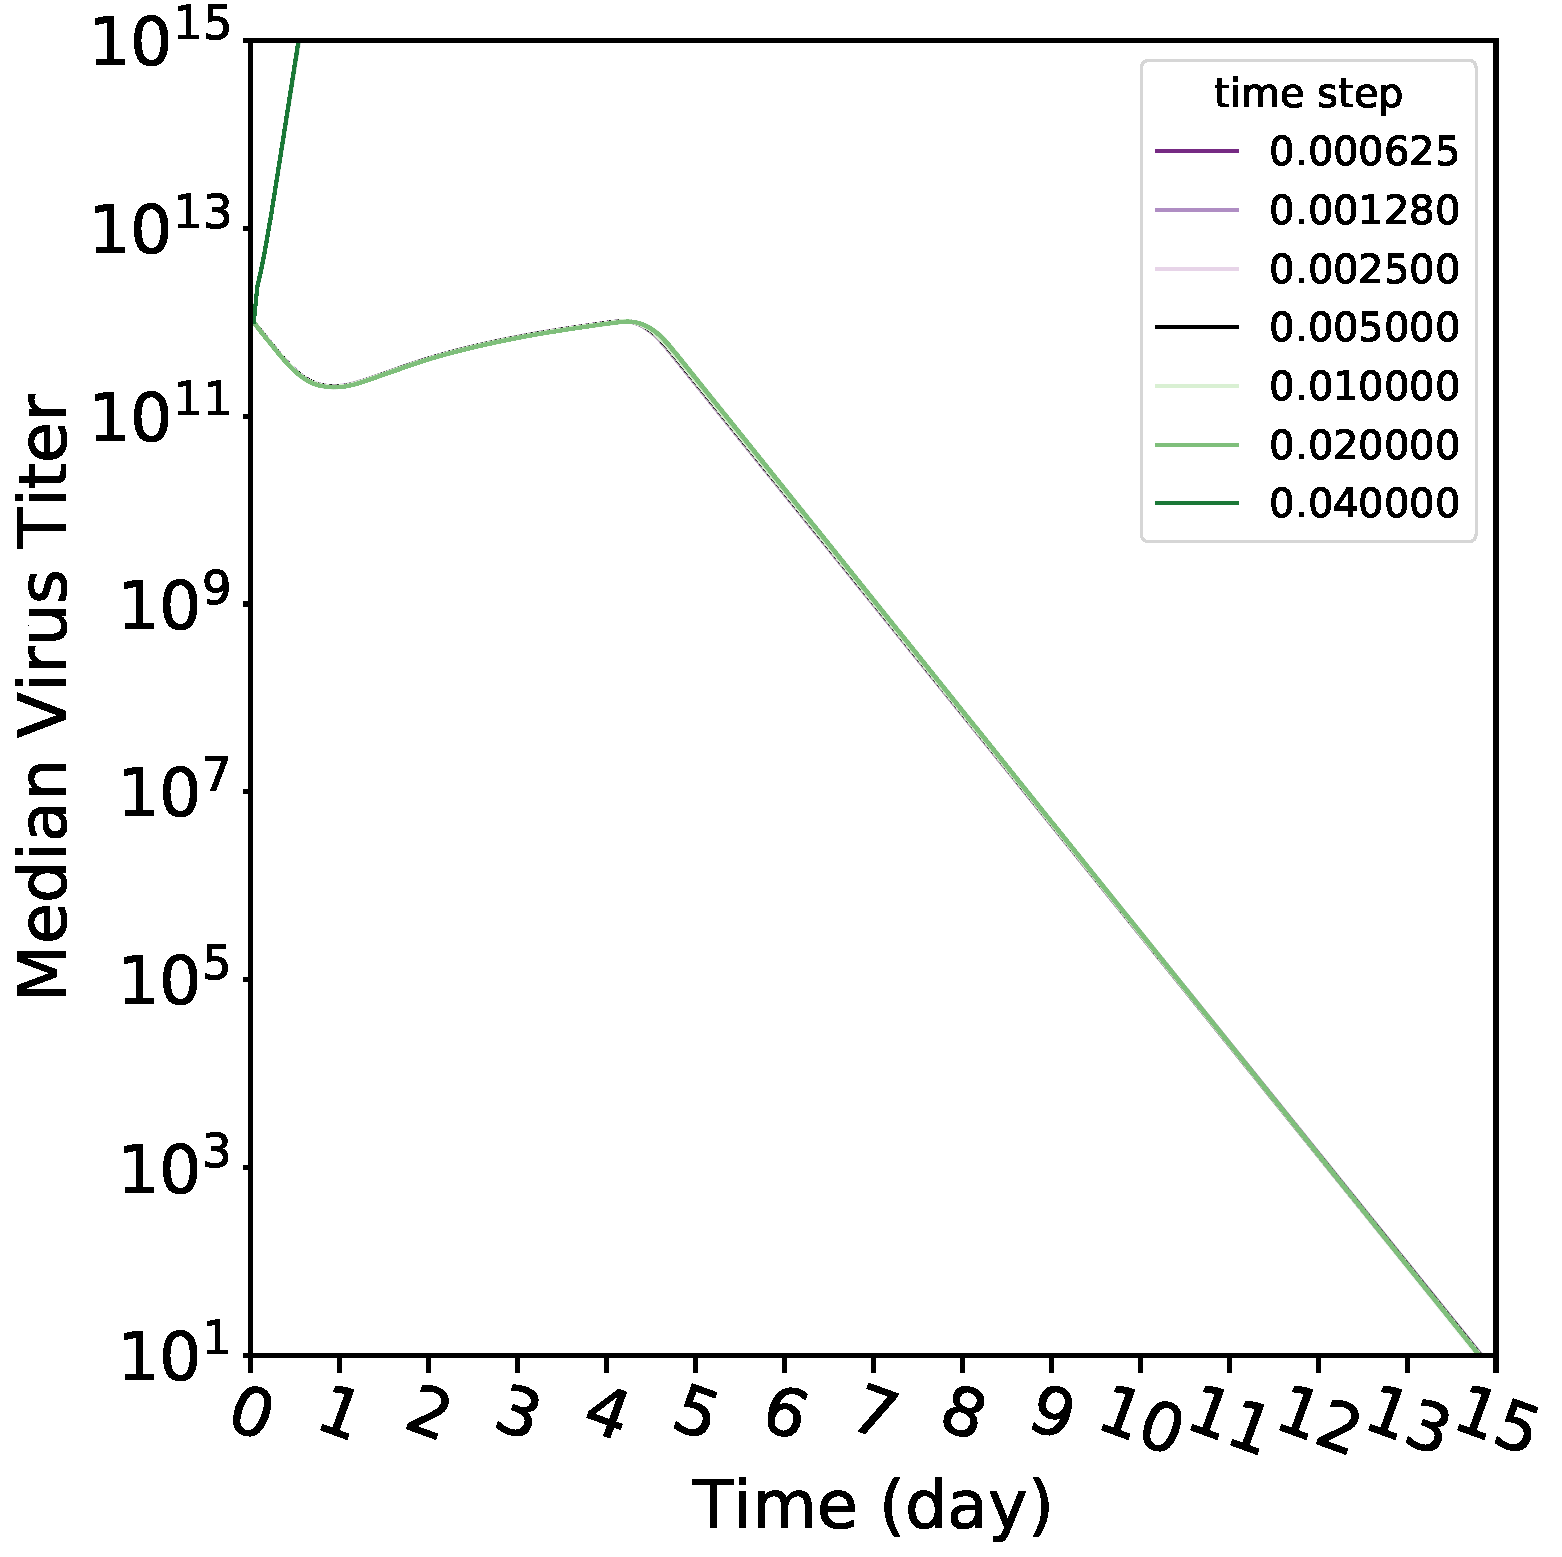
\includegraphics[width=0.33\linewidth]{Figures/Cellfree-InitialVirus-AllOnOne_Median_VirusVsTime.pdf}
        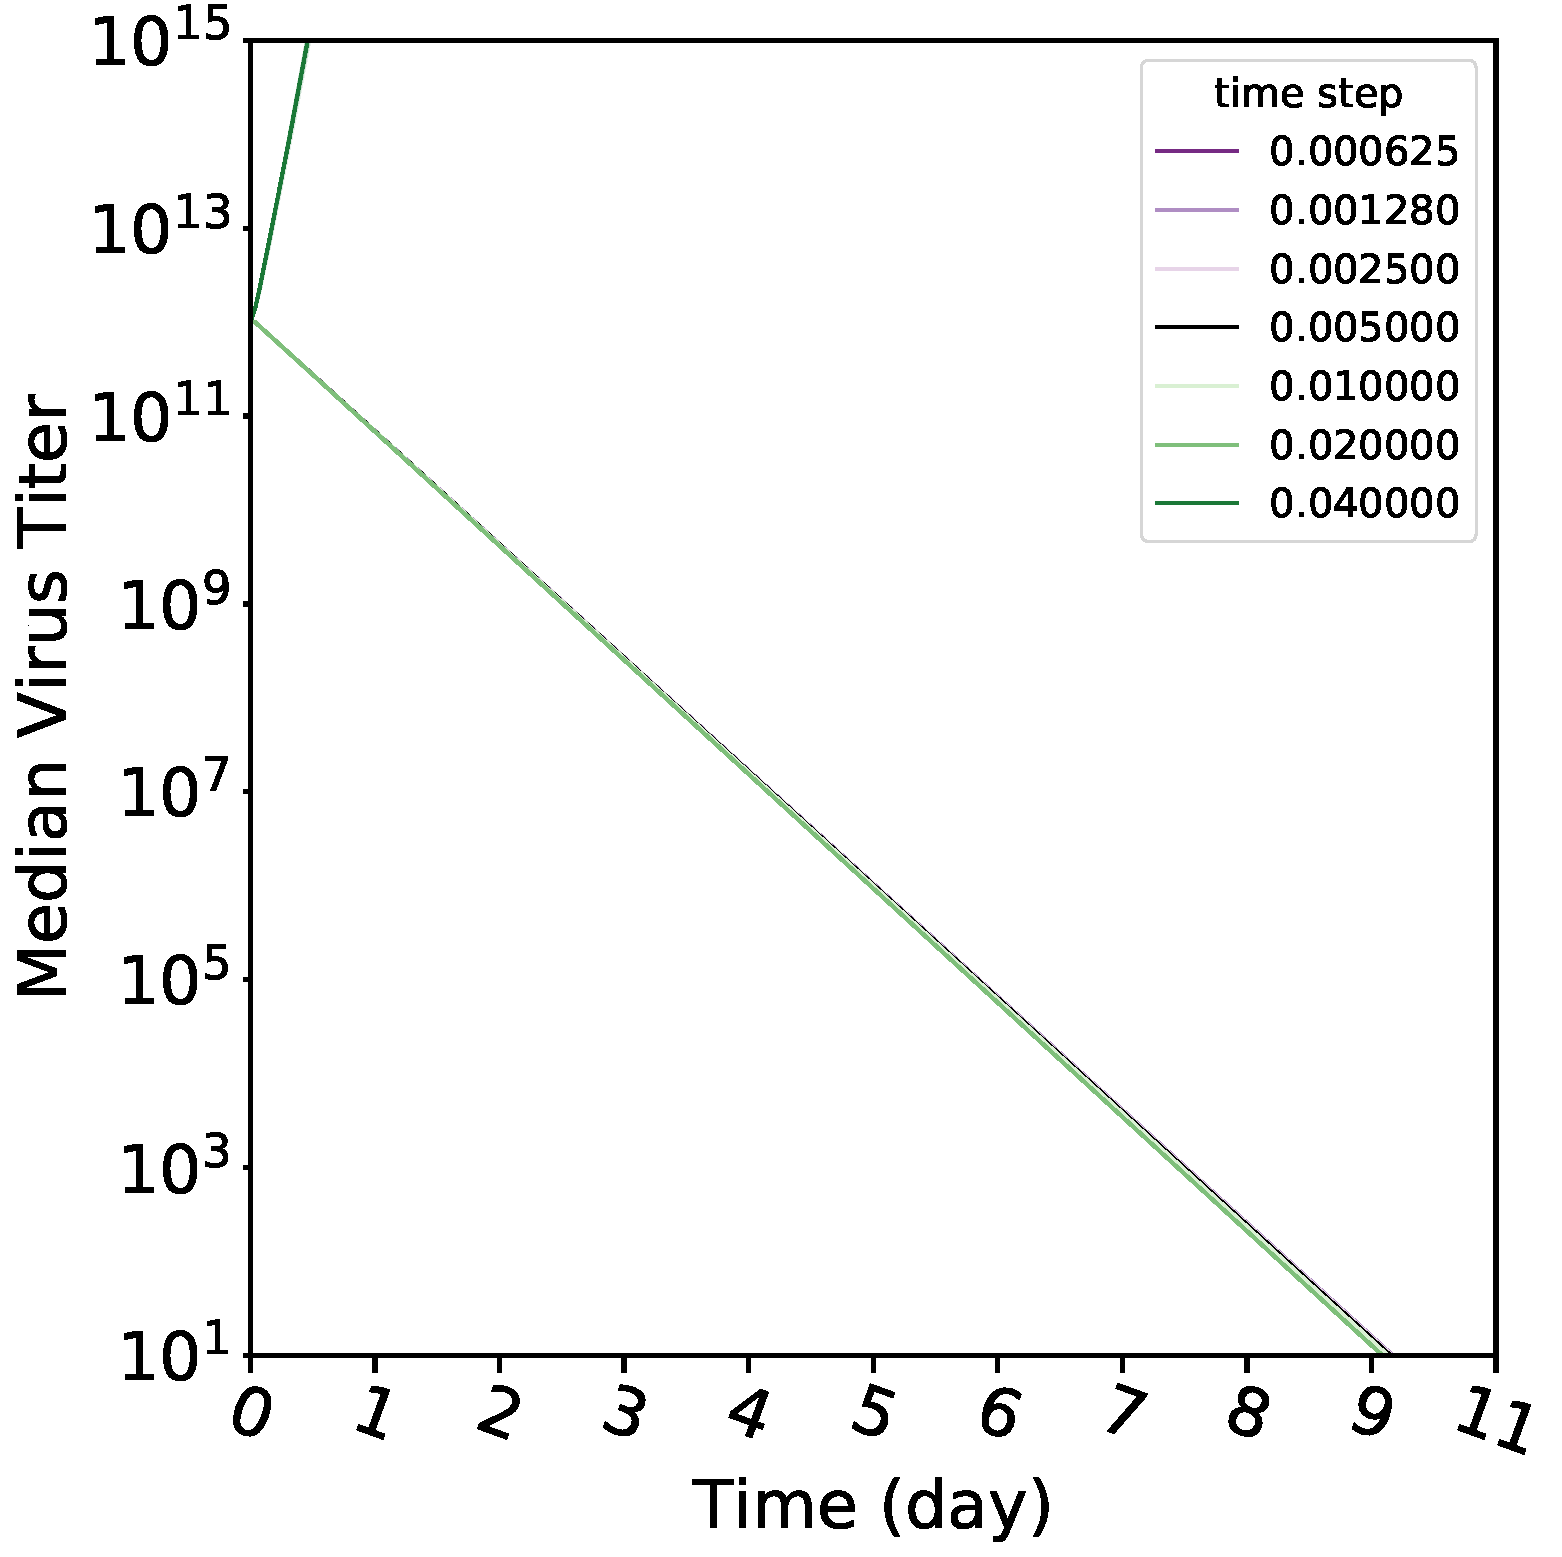
\includegraphics[width=0.33\linewidth]{Figures/Neither-InitialVirus-AllOnOne_Median_VirusVsTime.pdf}}}


\caption{The time step was varied to test the convergence of the model in time. A time step of 0.005 hr was chosen and a range around it was made by dividing or multiplying by 2 repeatedly. Seven values were used [0.000625, 0.00128, 0.0025, 0.005, 0.01, 0.02, 0.04]. The median curve of ten viral titer curves is shown for each time step. From left to right, curves of a viral infection exhibiting cell-free transmission initiated with infected cells; curves of a viral infection exhibiting cell-free transmission initiated with virus; and curves of virus without underlying cell infection. \label{fig:ViralTiterCurves}}
\end{figure}

In figure \ref{fig_AspectGraphs} the different viral titer curves are explored further by plotting the measurable characteristics mentioned in section \ref{convergence_measures} for each time step. For all the characteristics, except AUC, the amount of change was in the hundredths place or less, so for time characteristics the amount of change was less than \SI{14.5}{\minute}, for 1/time characteristics the amount of change was less than \SI{6.9e-6}{\per\minute}, and for amount of virus characteristics the amount of change was less than \num{e10} virus particles, which is less than \SI{1}{\percent} change in the amount of virus. Note that typical experimental error in measurements of viral load are typically 0.5 $\log_{10}$(PFU/ml) \citep{labarre01}. The AUC varied the most over the different timesteps. The mean of the AUC values for the different timesteps is \SI{3626}{log(virus)\per\day} with a standard deviation (STD) of \SI{13.09}{log(virus)\per\day}. Therefore, the coefficient of variation is $CV = \frac{13.09}{3626} \approx 0.0036$, which shows that the STD is about \SI{0.36}{\percent} the size of the mean.

\begin{figure}
\centering
\begin{minipage}{\linewidth}
    \centering
    \parbox{\textwidth}{
    \fbox{\parbox{\textwidth}{\vspace{-1em}
    \begin{multicols}{3}
        \centering

        Initial Cell

        Initial Virus

        Only Virus
    \end{multicols}
    \vspace{-1em}}}

    \vspace{0.5em}
    \centering
    \resizebox{\textwidth}{!}{%
    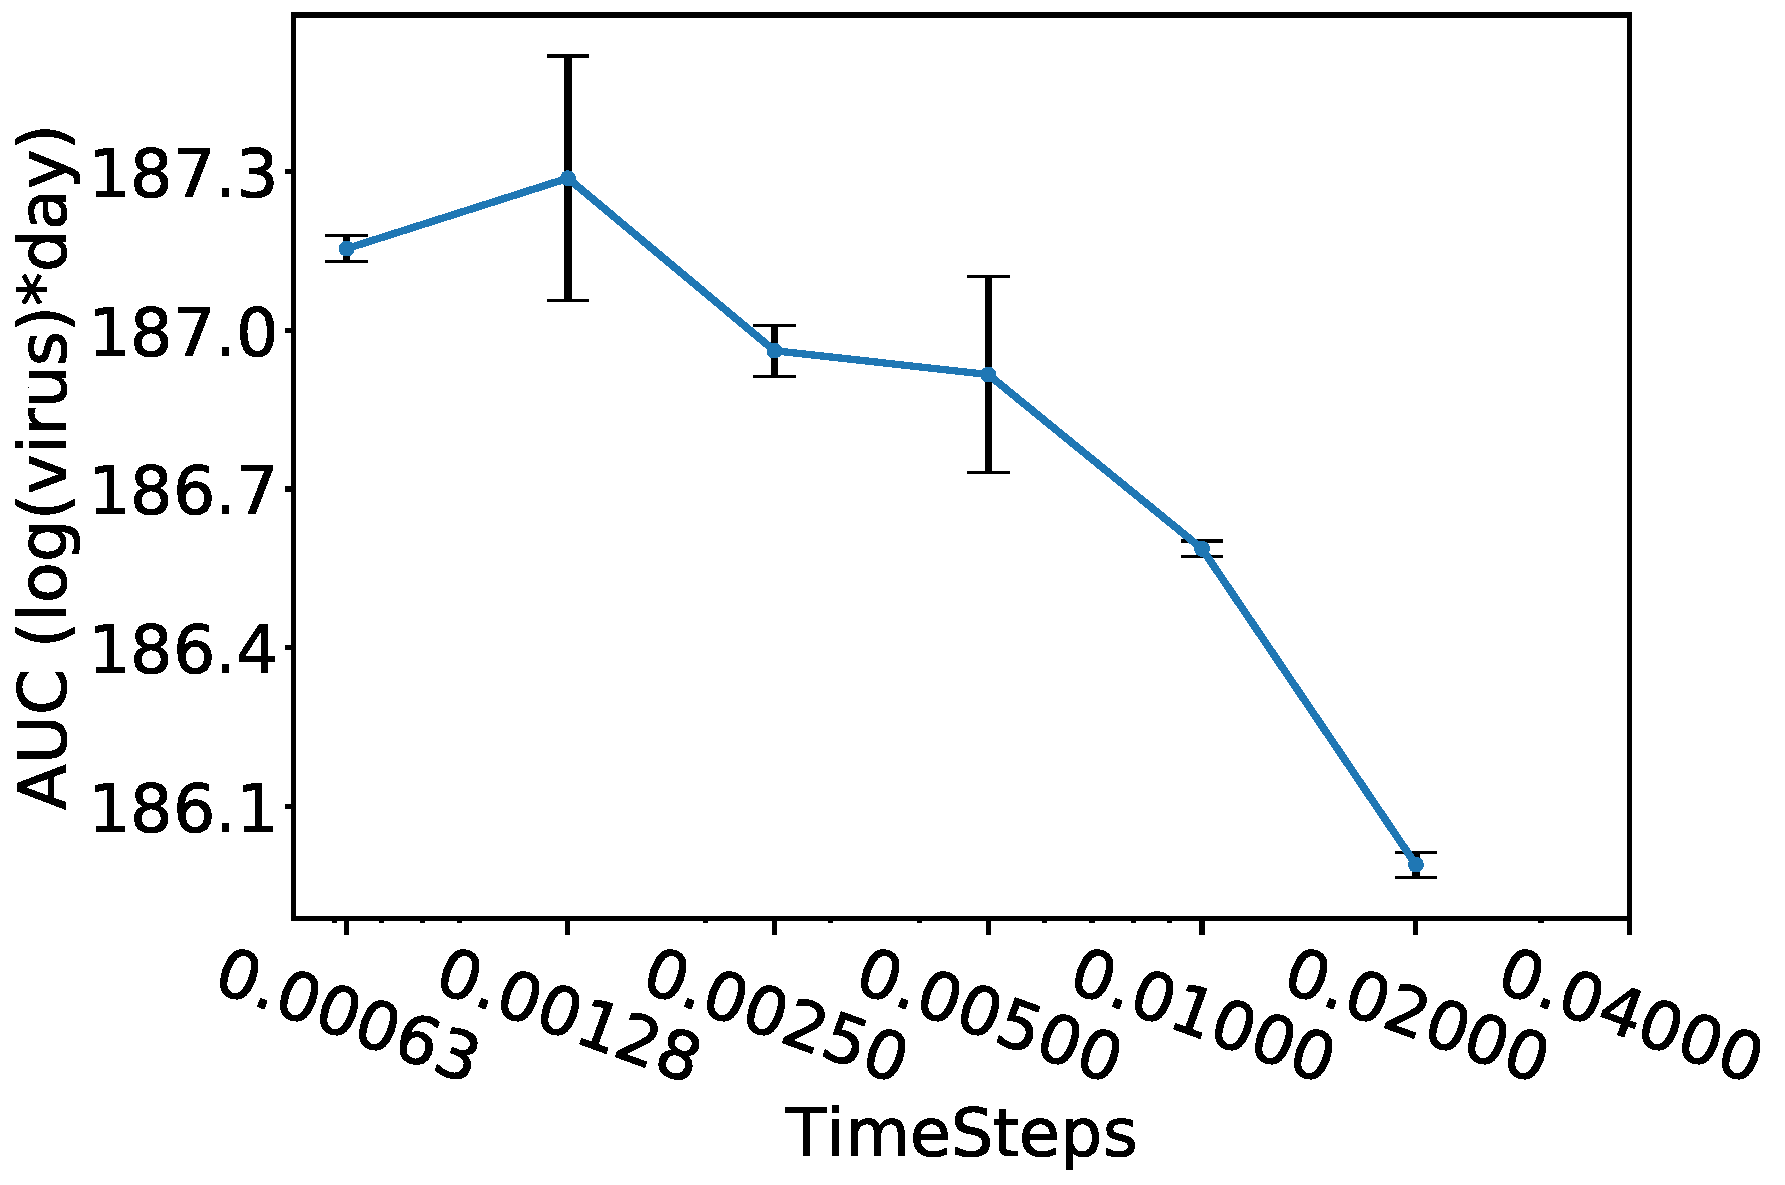
\includegraphics[width=0.33\linewidth]{Figures/Cellfree-InitialCell-Runs_Graphs/AUC.pdf}
    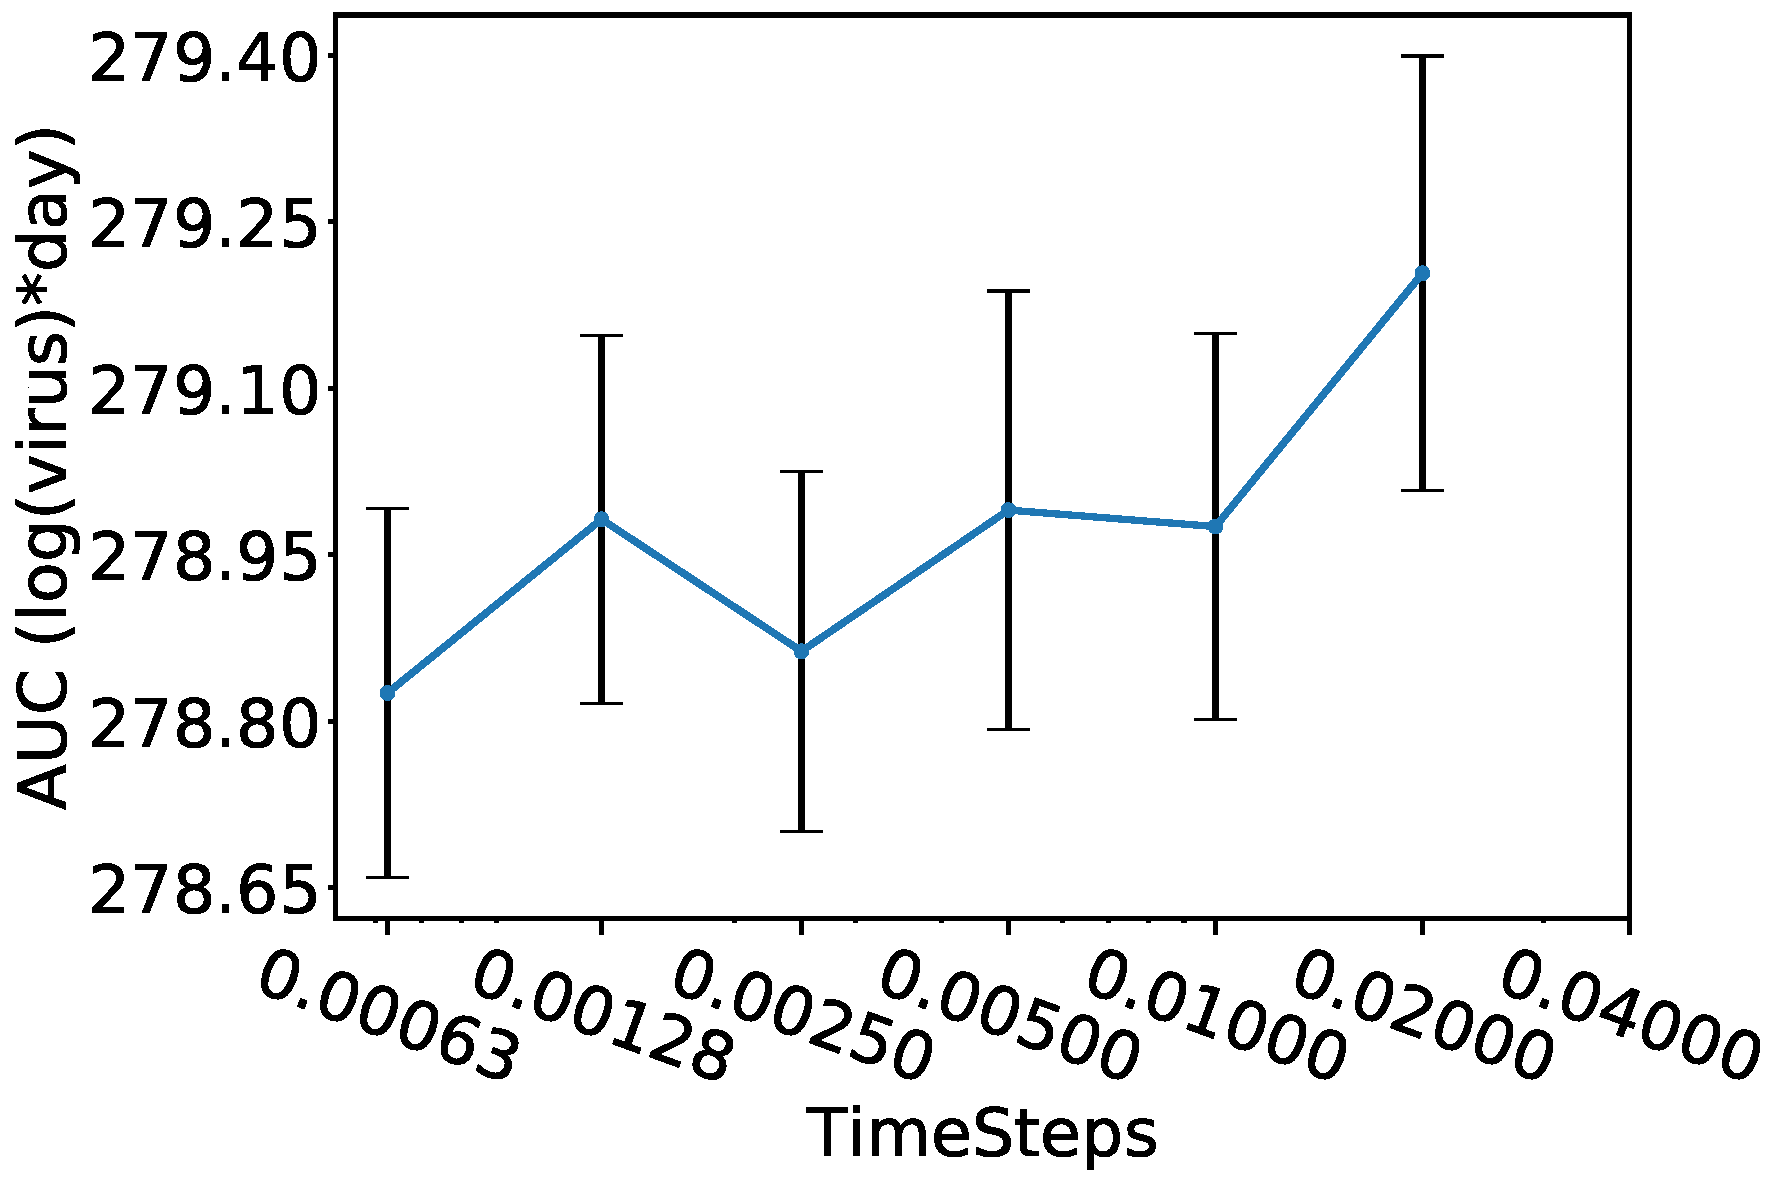
\includegraphics[width=0.33\linewidth]{Figures/Cellfree-InitialVirus-Runs_Graphs/AUC.pdf}
    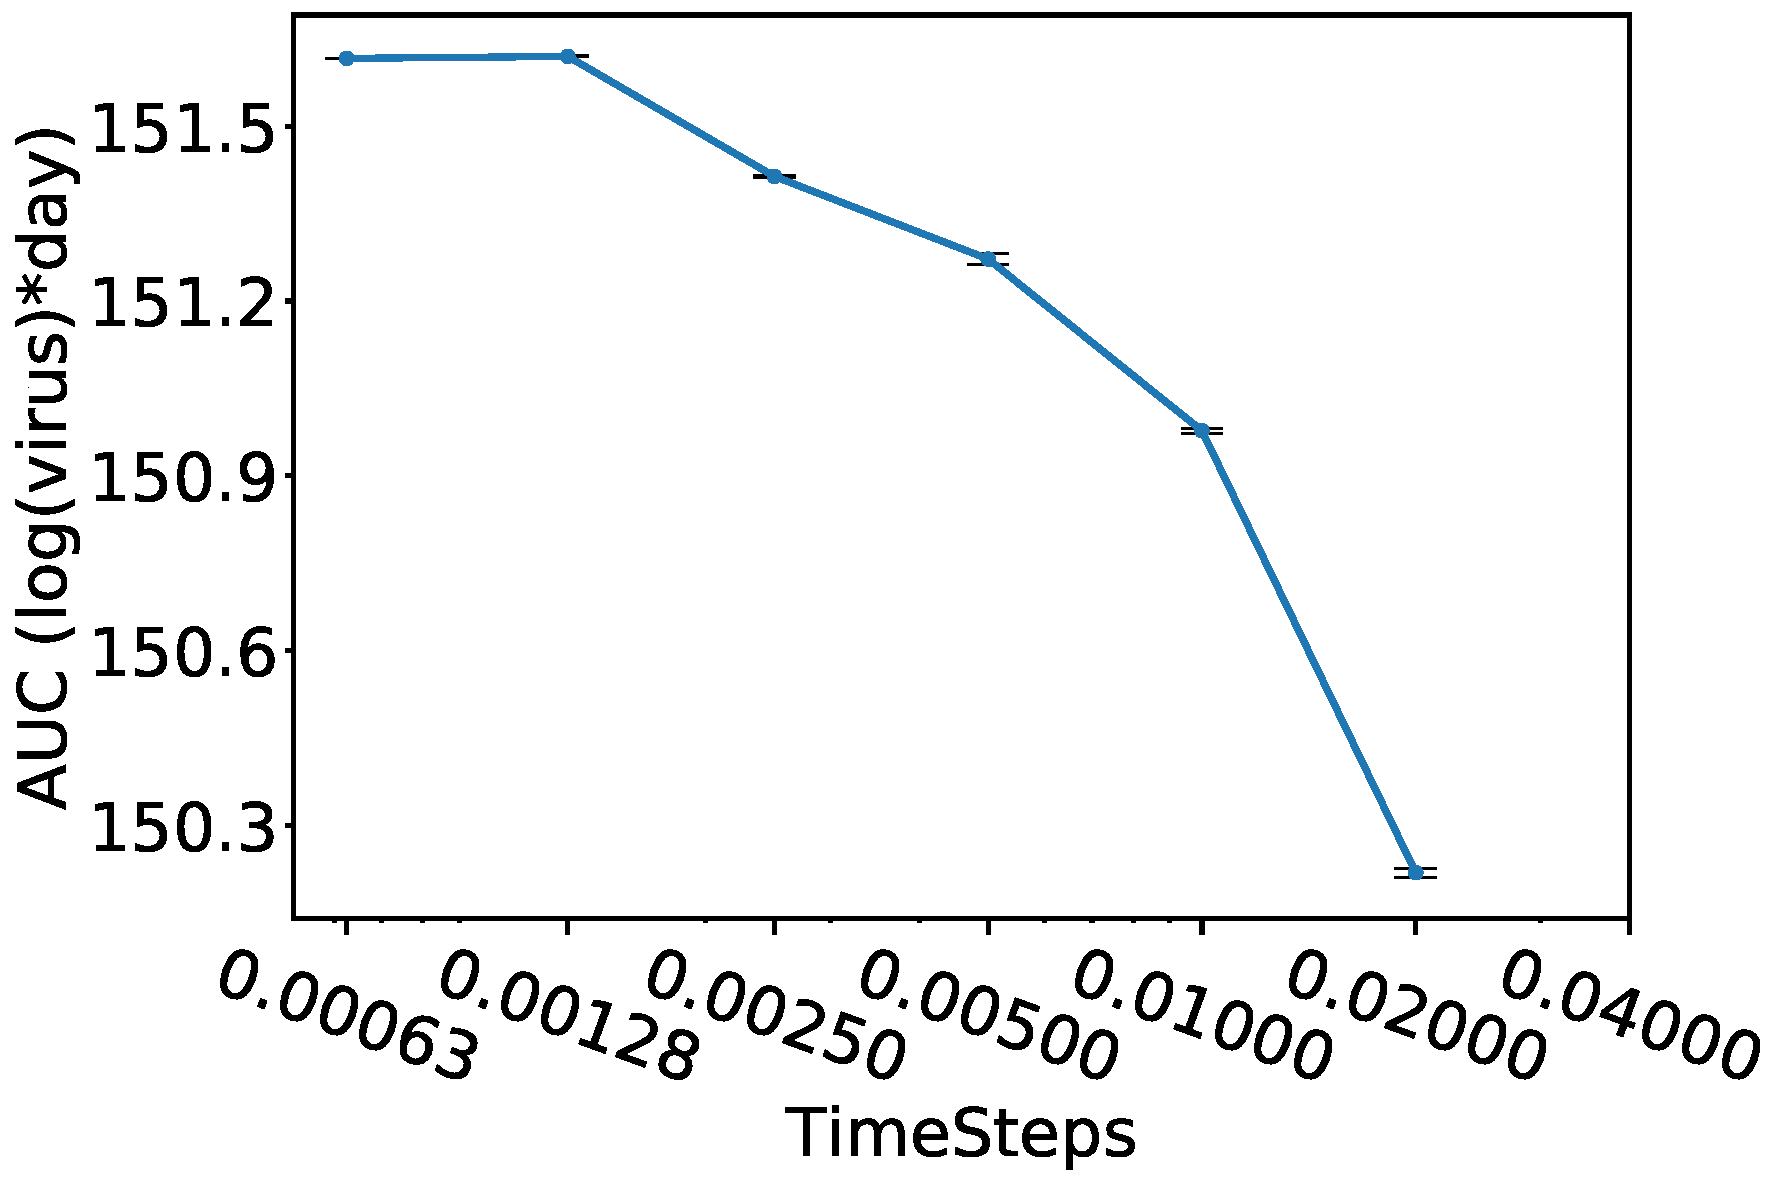
\includegraphics[width=0.33\linewidth]{Figures/Neither-InitialVirus-Runs_Graphs/AUC.pdf}}


    \resizebox{\textwidth}{!}{%
    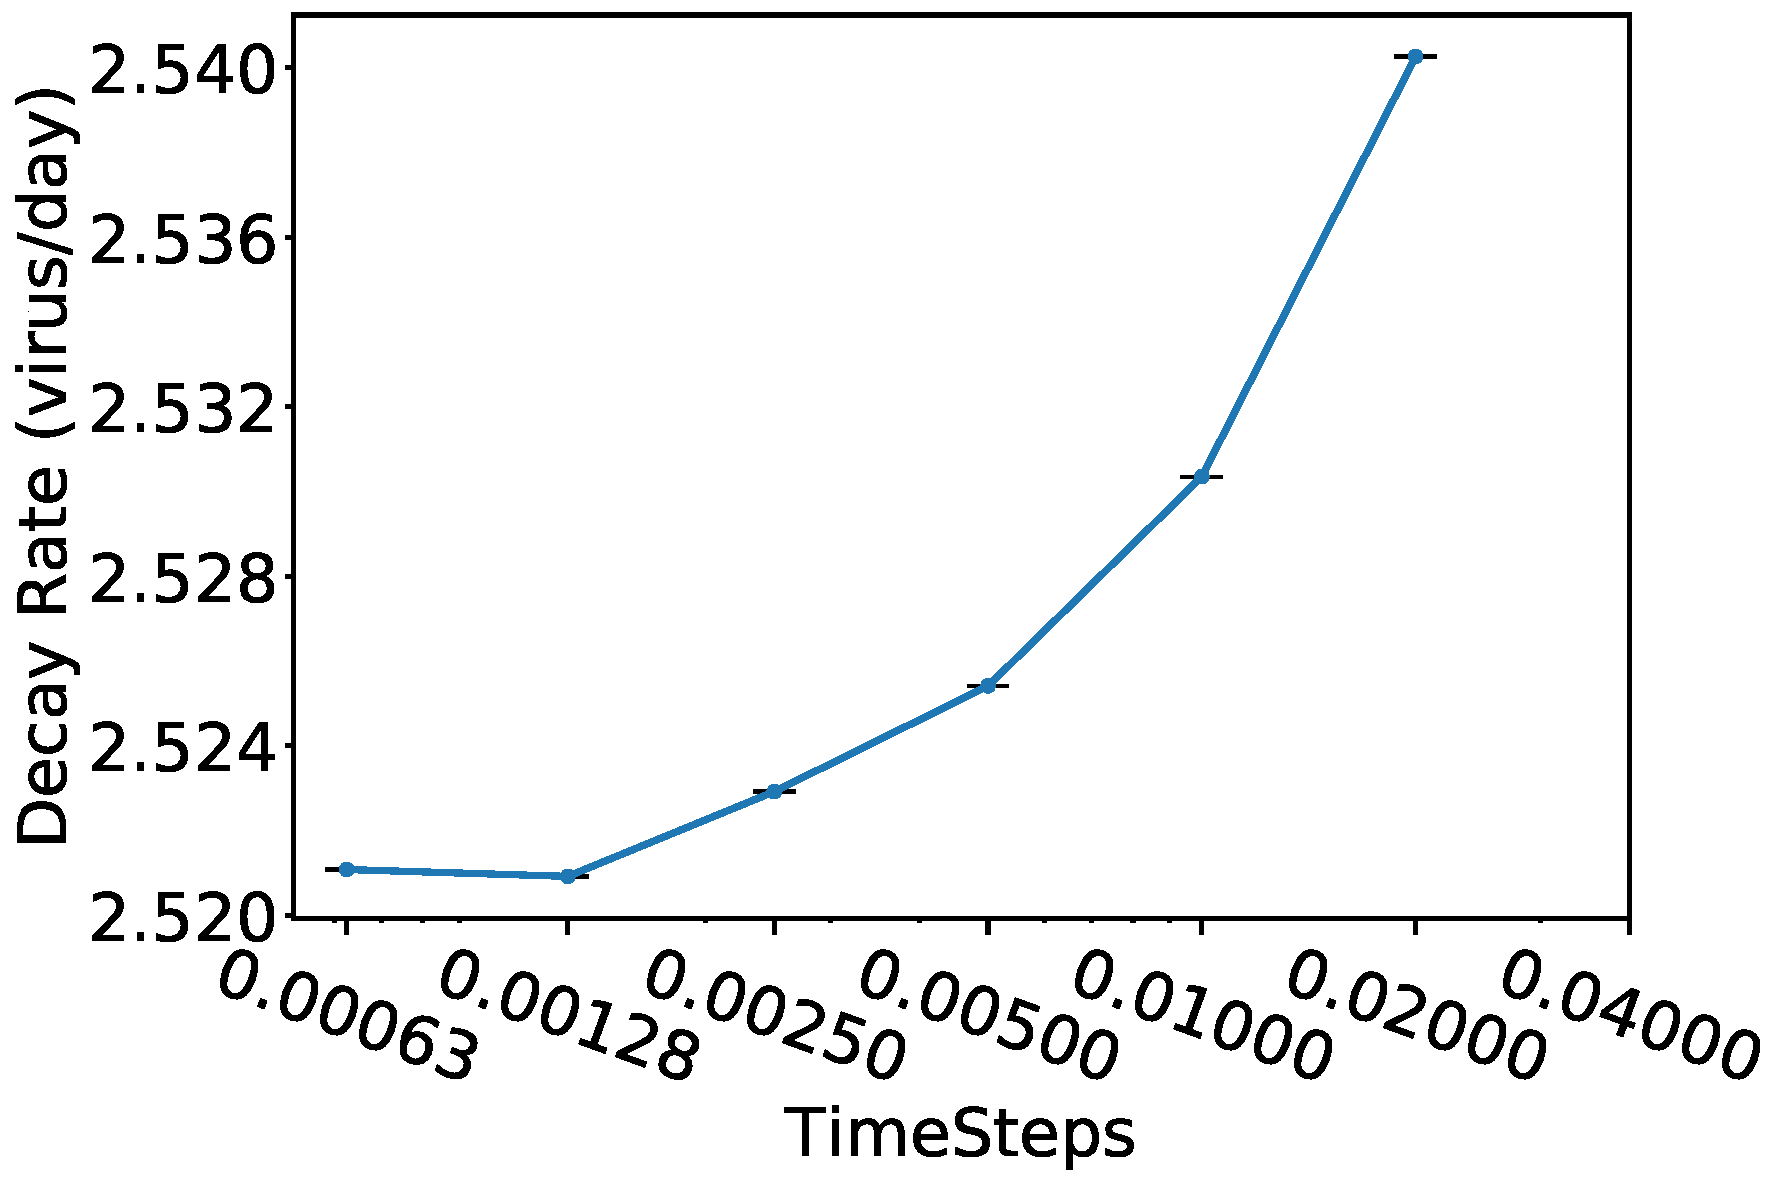
\includegraphics[width=0.33\linewidth]{Figures/Cellfree-InitialCell-Runs_Graphs/DownSlope.pdf}
    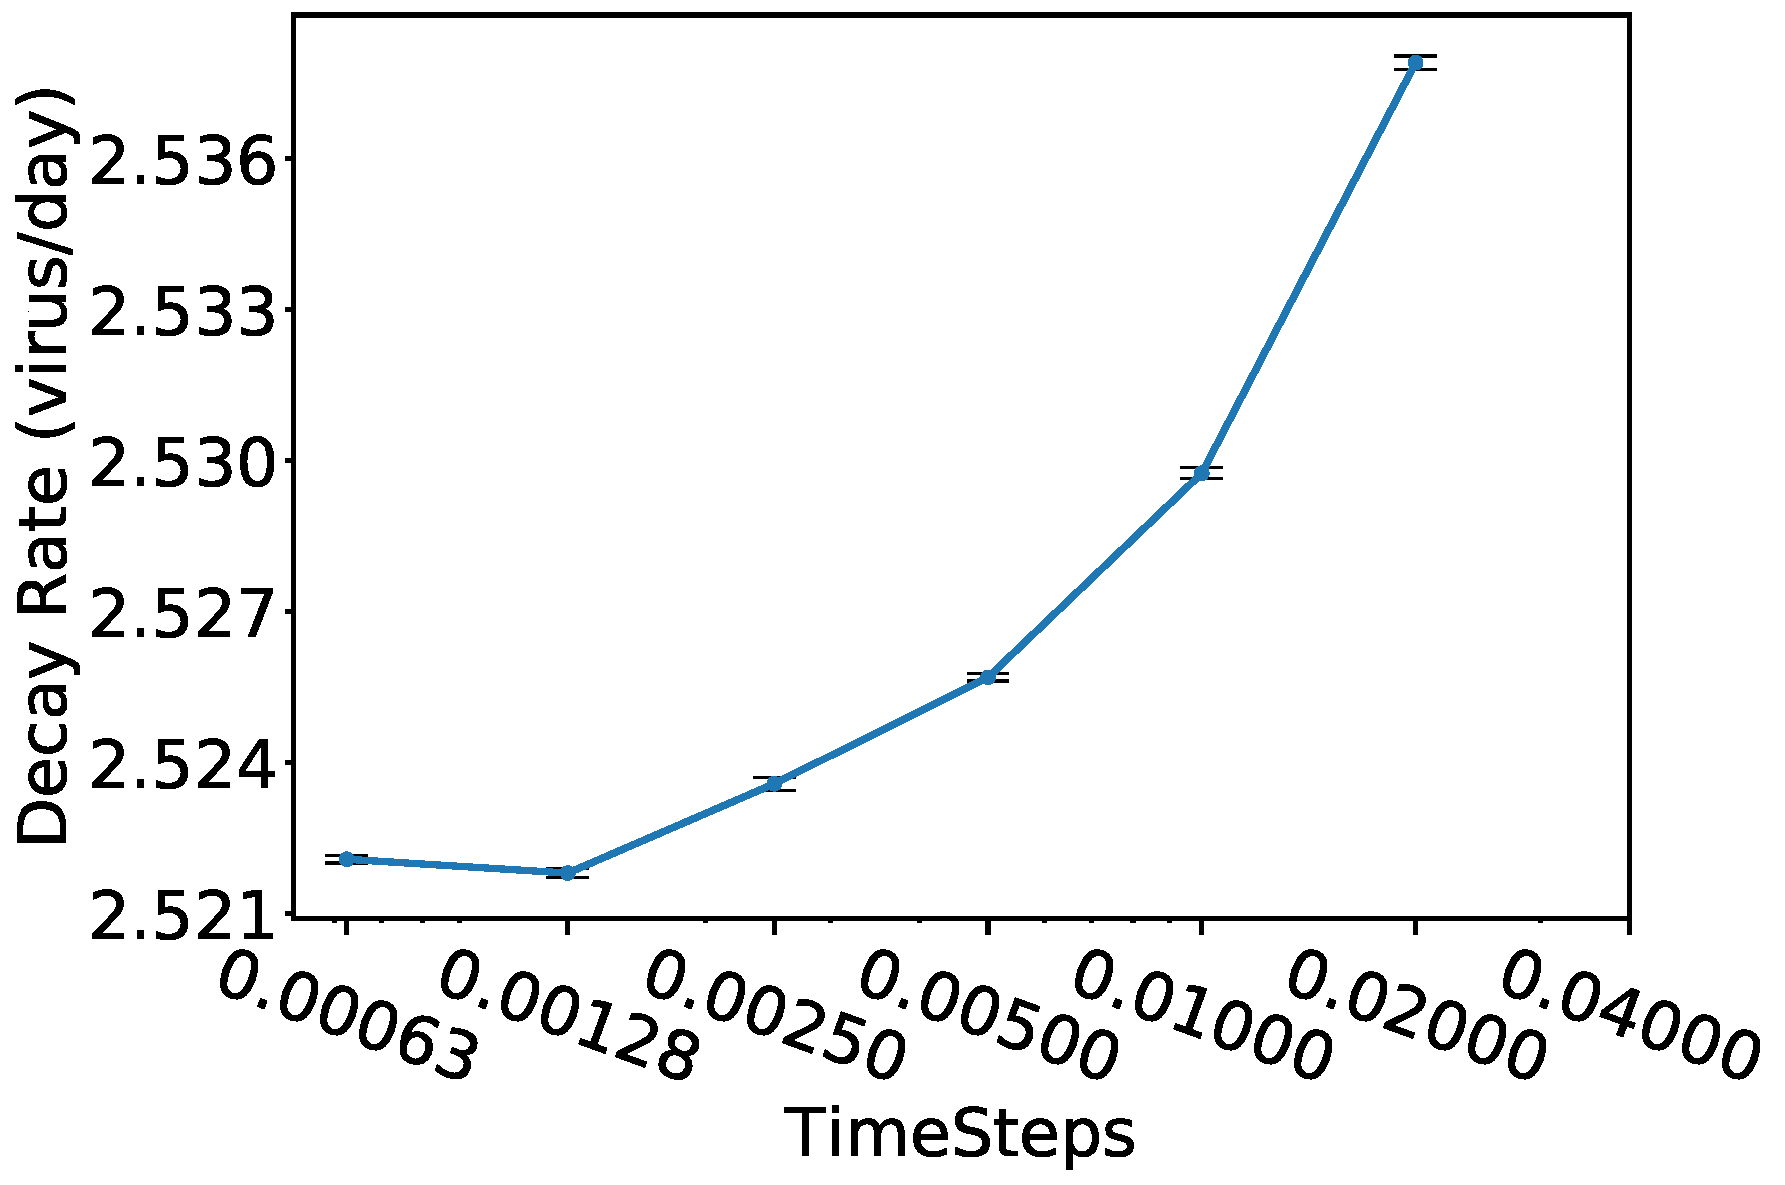
\includegraphics[width=0.33\linewidth]{Figures/Cellfree-InitialVirus-Runs_Graphs/DownSlope.pdf}
    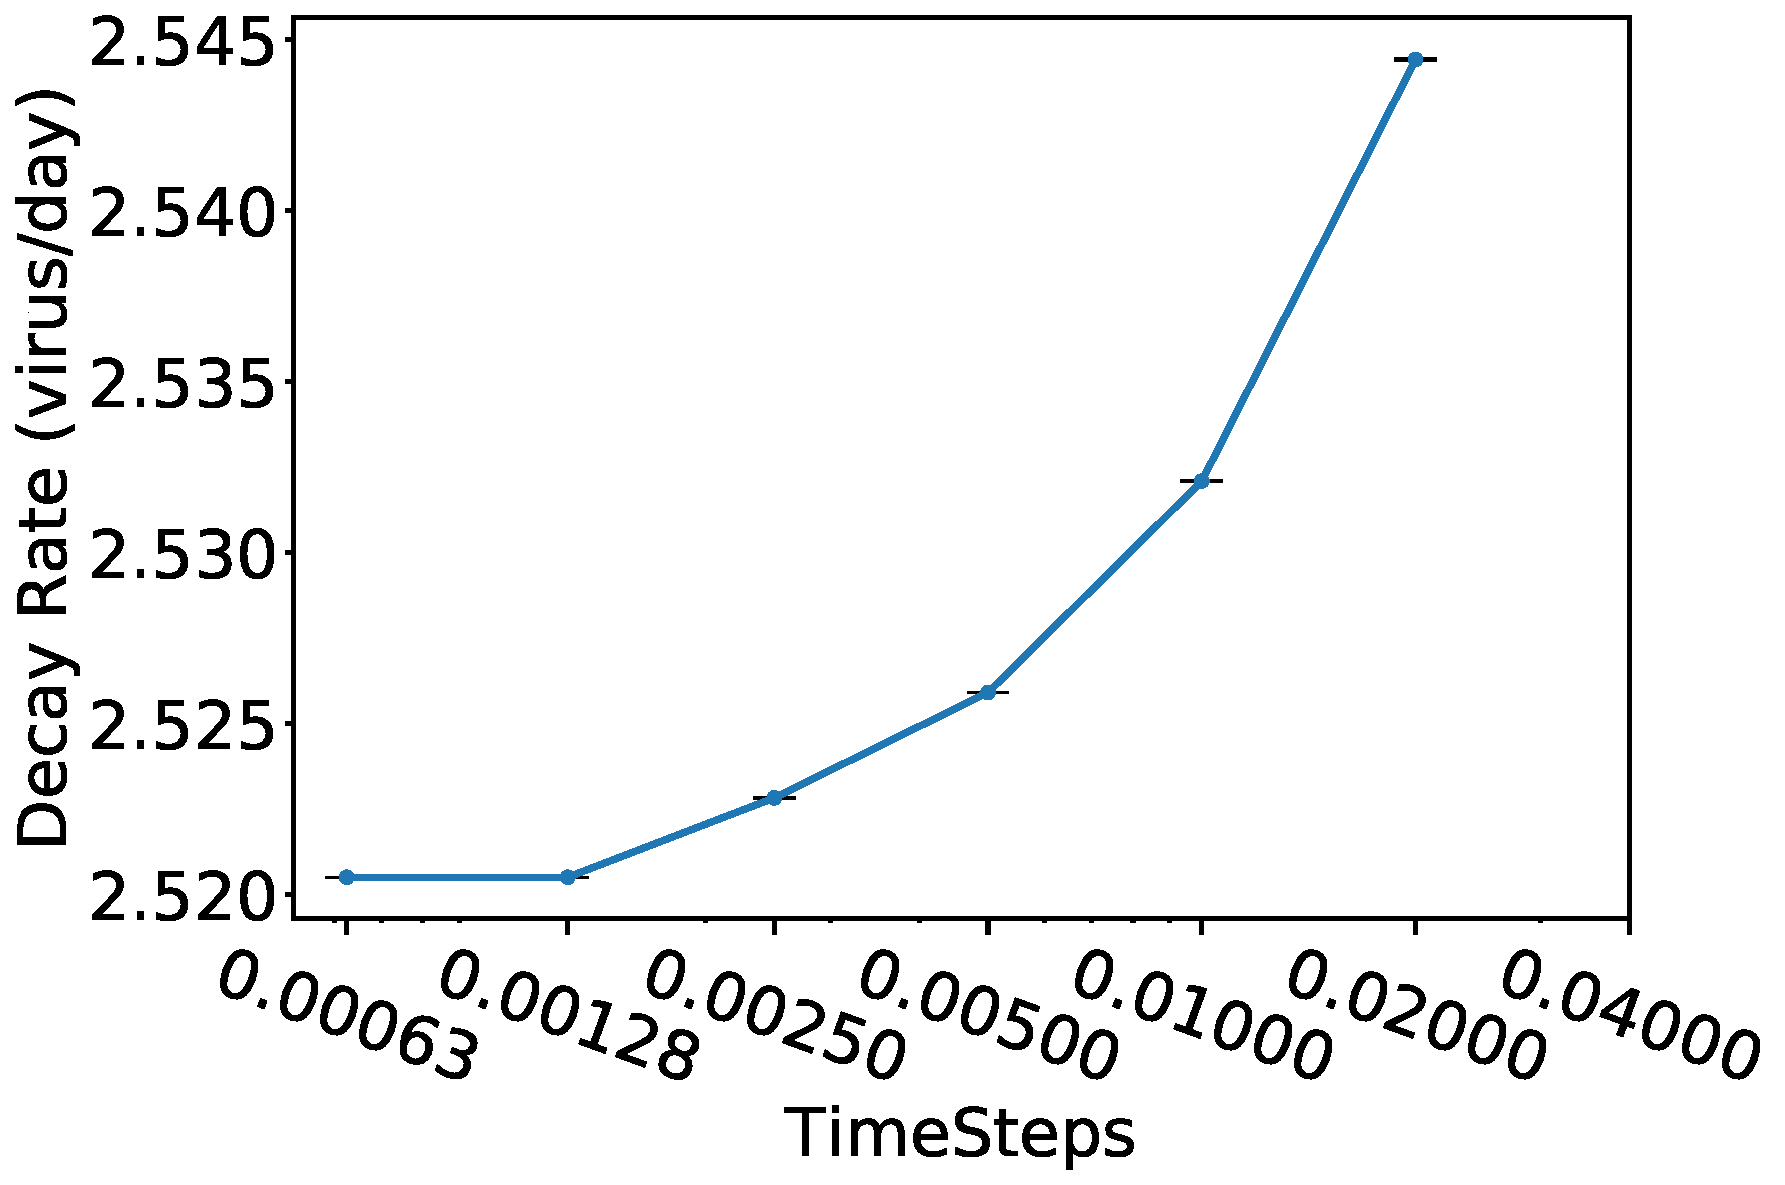
\includegraphics[width=0.33\linewidth]{Figures/Neither-InitialVirus-Runs_Graphs/DownSlope.pdf}}

    \resizebox{\textwidth}{!}{%
    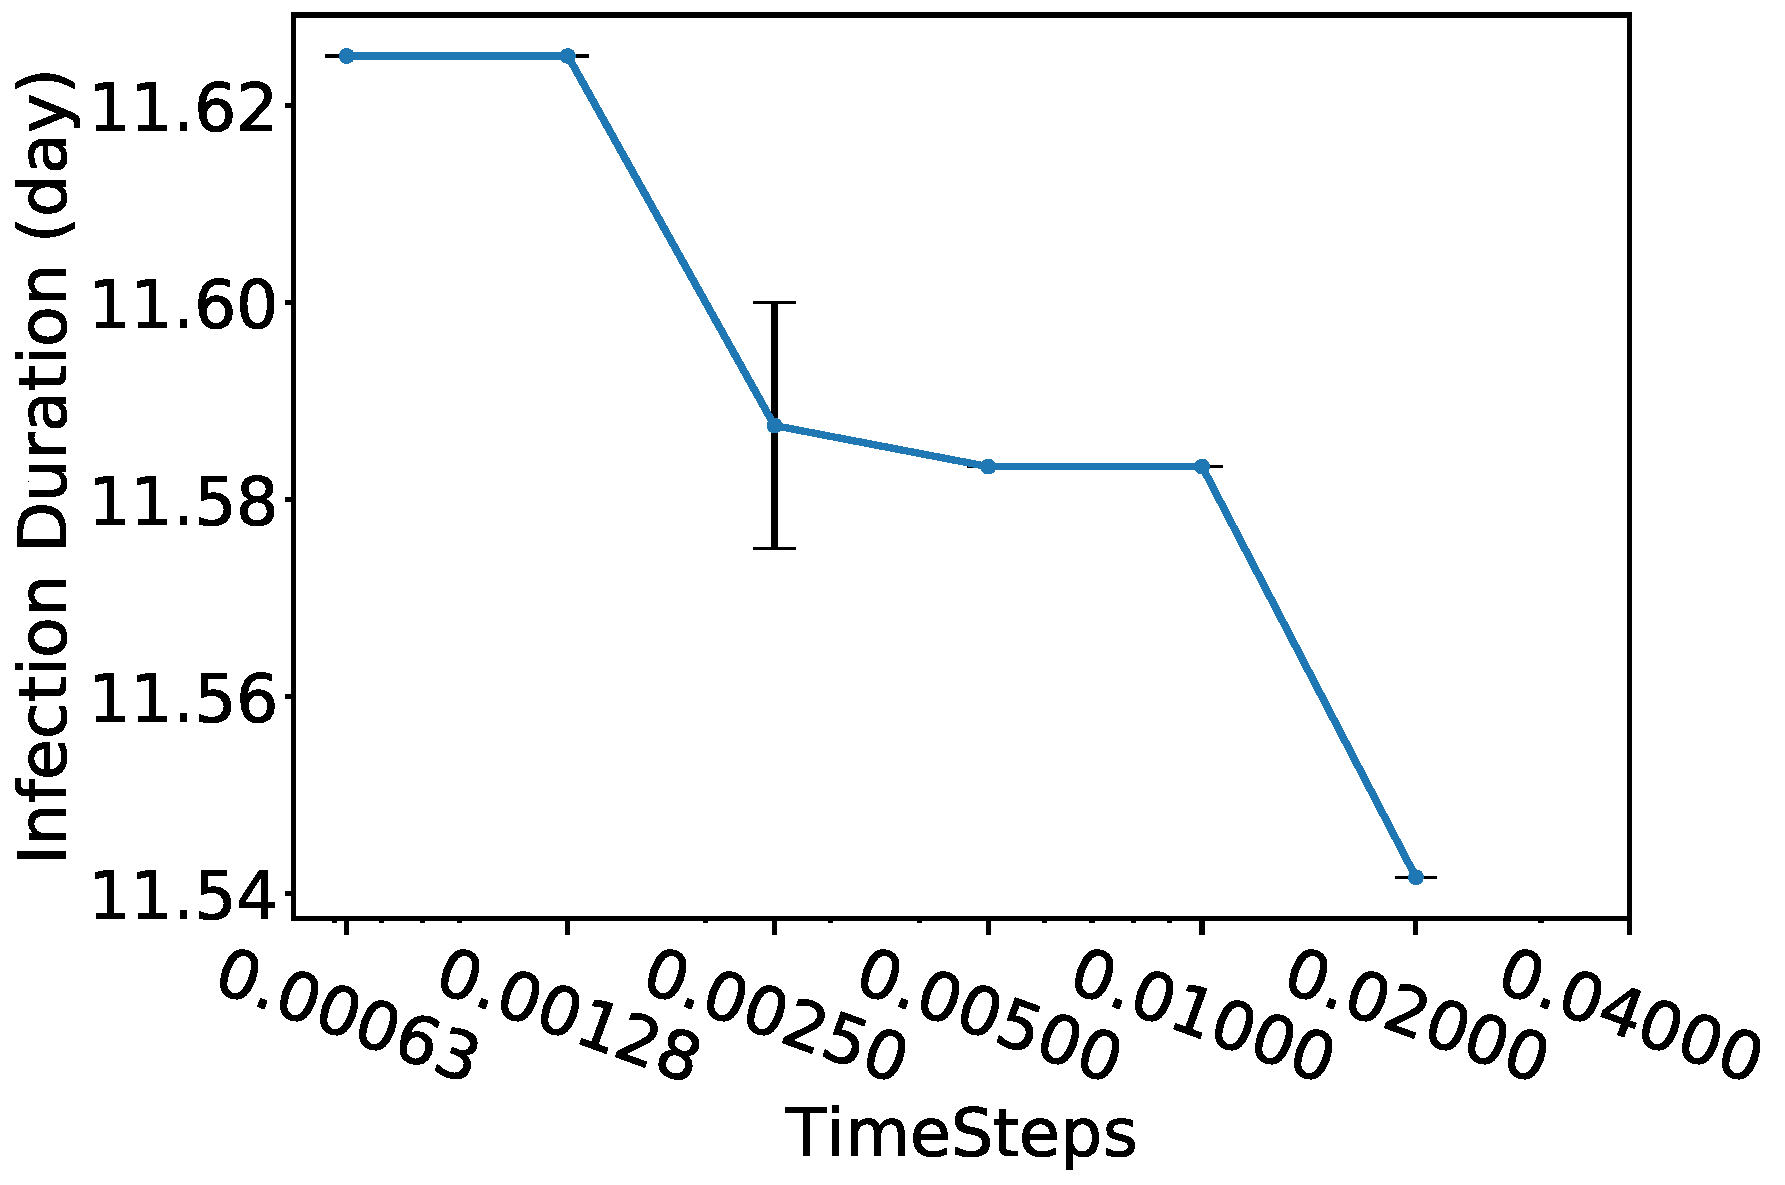
\includegraphics[width=0.33\linewidth]{Figures/Cellfree-InitialCell-Runs_Graphs/InfectionDuration.pdf}
    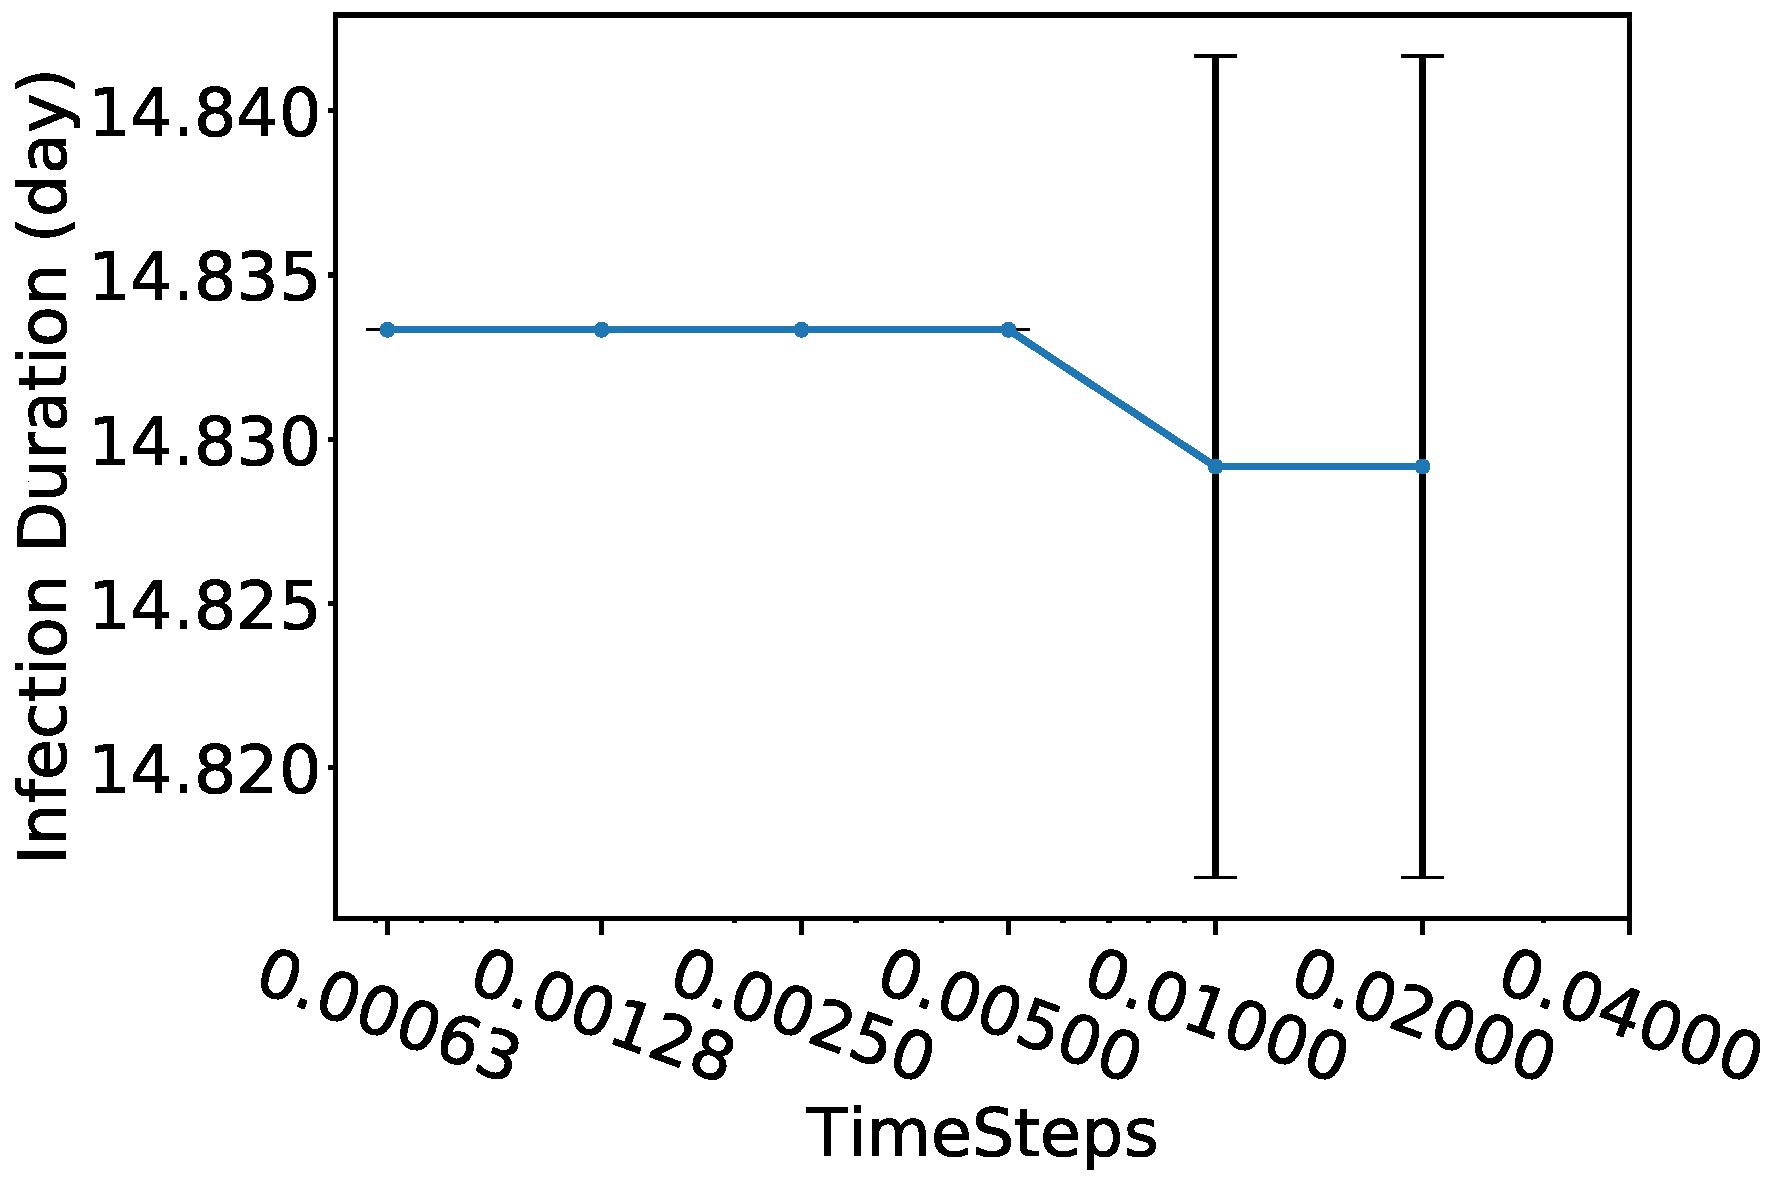
\includegraphics[width=0.33\linewidth]{Figures/Cellfree-InitialVirus-Runs_Graphs/InfectionDuration.pdf}
    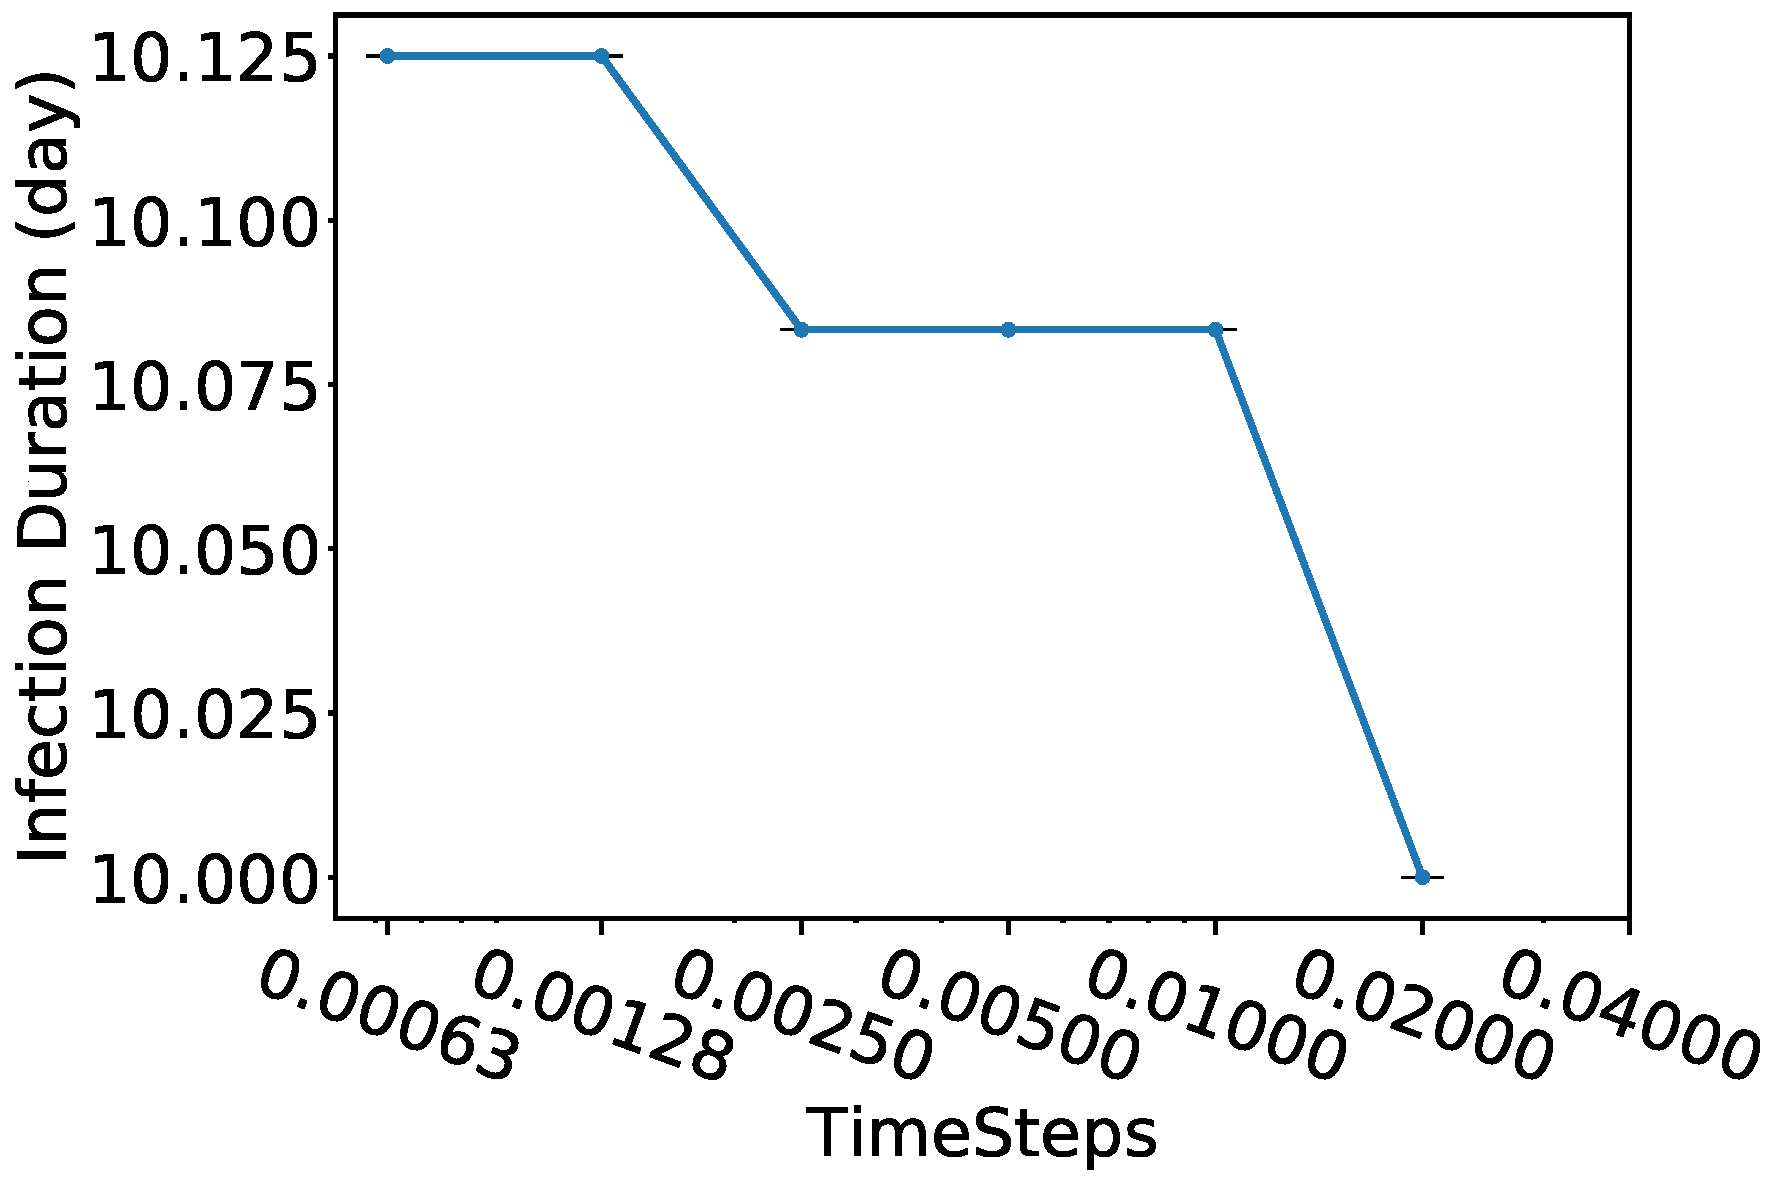
\includegraphics[width=0.33\linewidth]{Figures/Neither-InitialVirus-Runs_Graphs/InfectionDuration.pdf}}

    \resizebox{\textwidth}{!}{%
    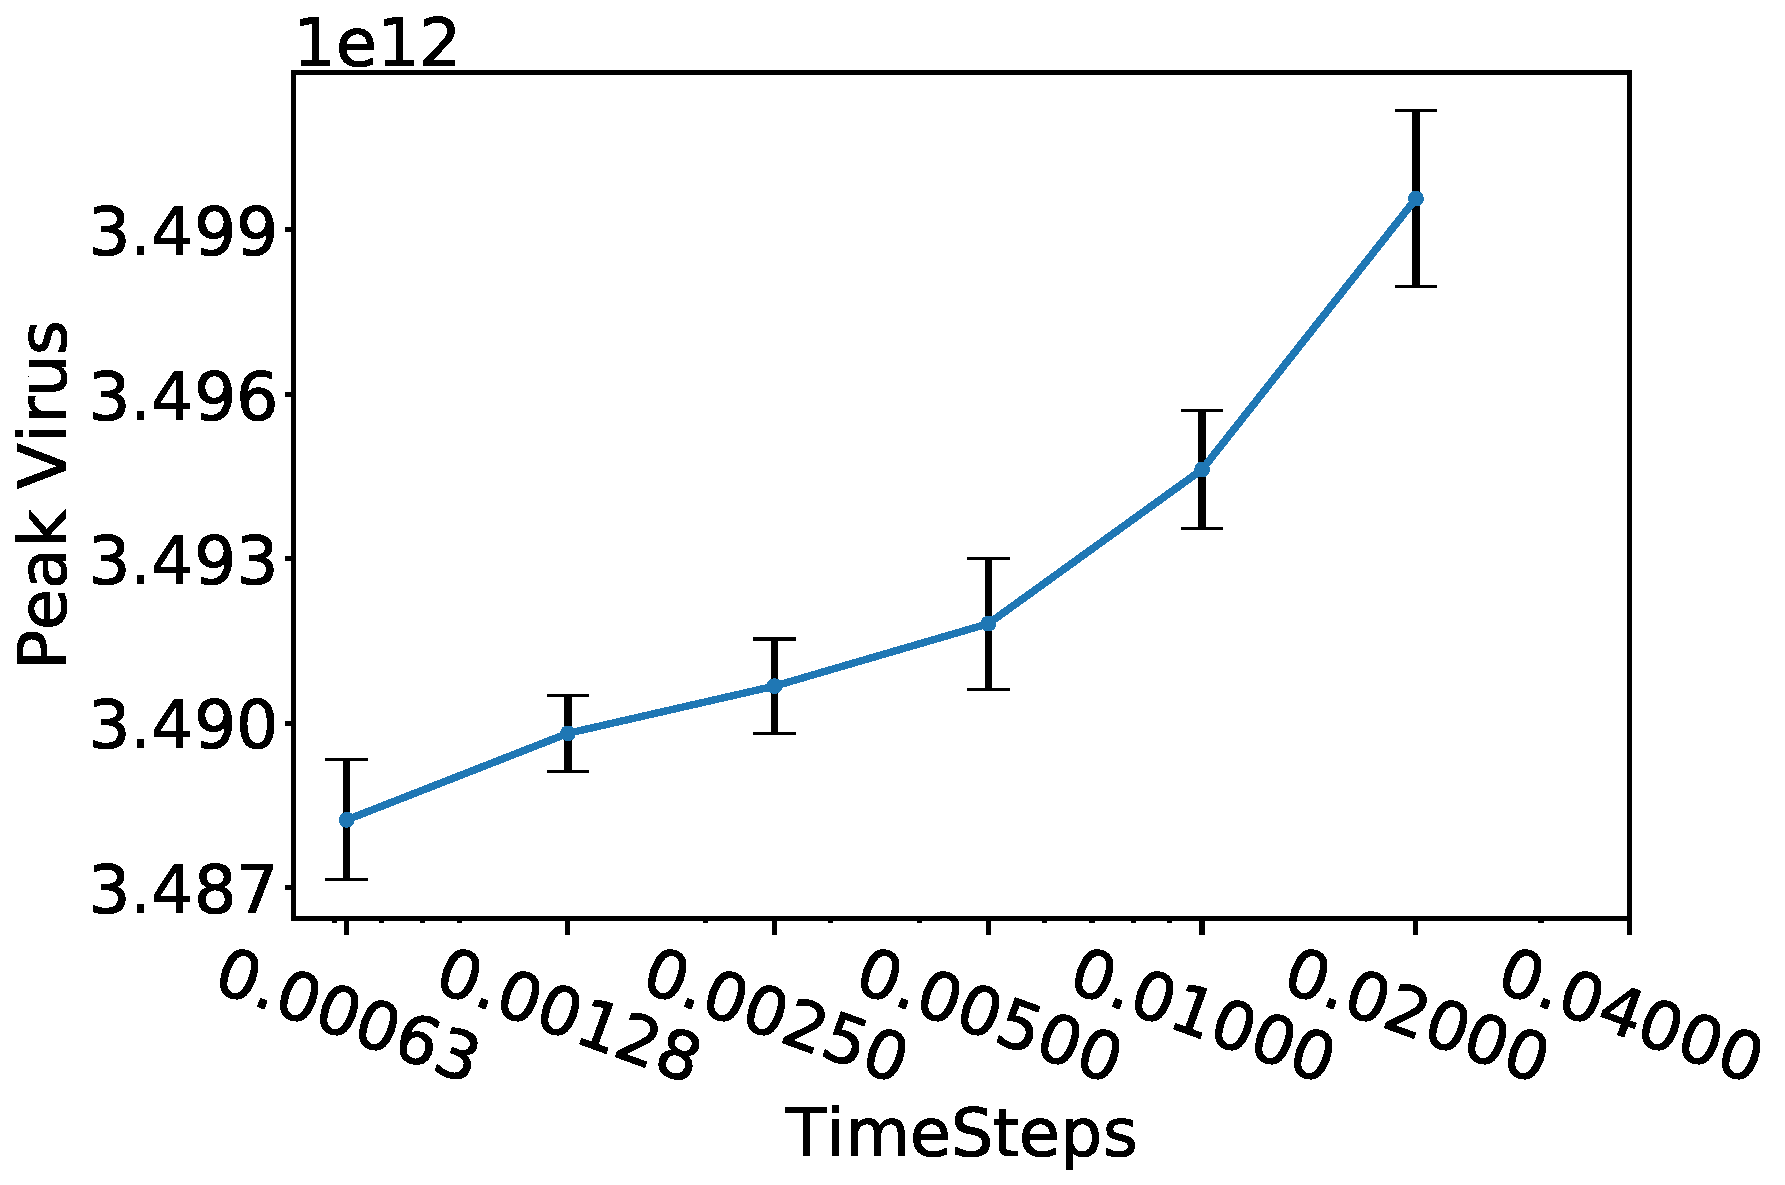
\includegraphics[width=0.33\linewidth]{Figures/Cellfree-InitialCell-Runs_Graphs/PeakViralTiter.pdf}
    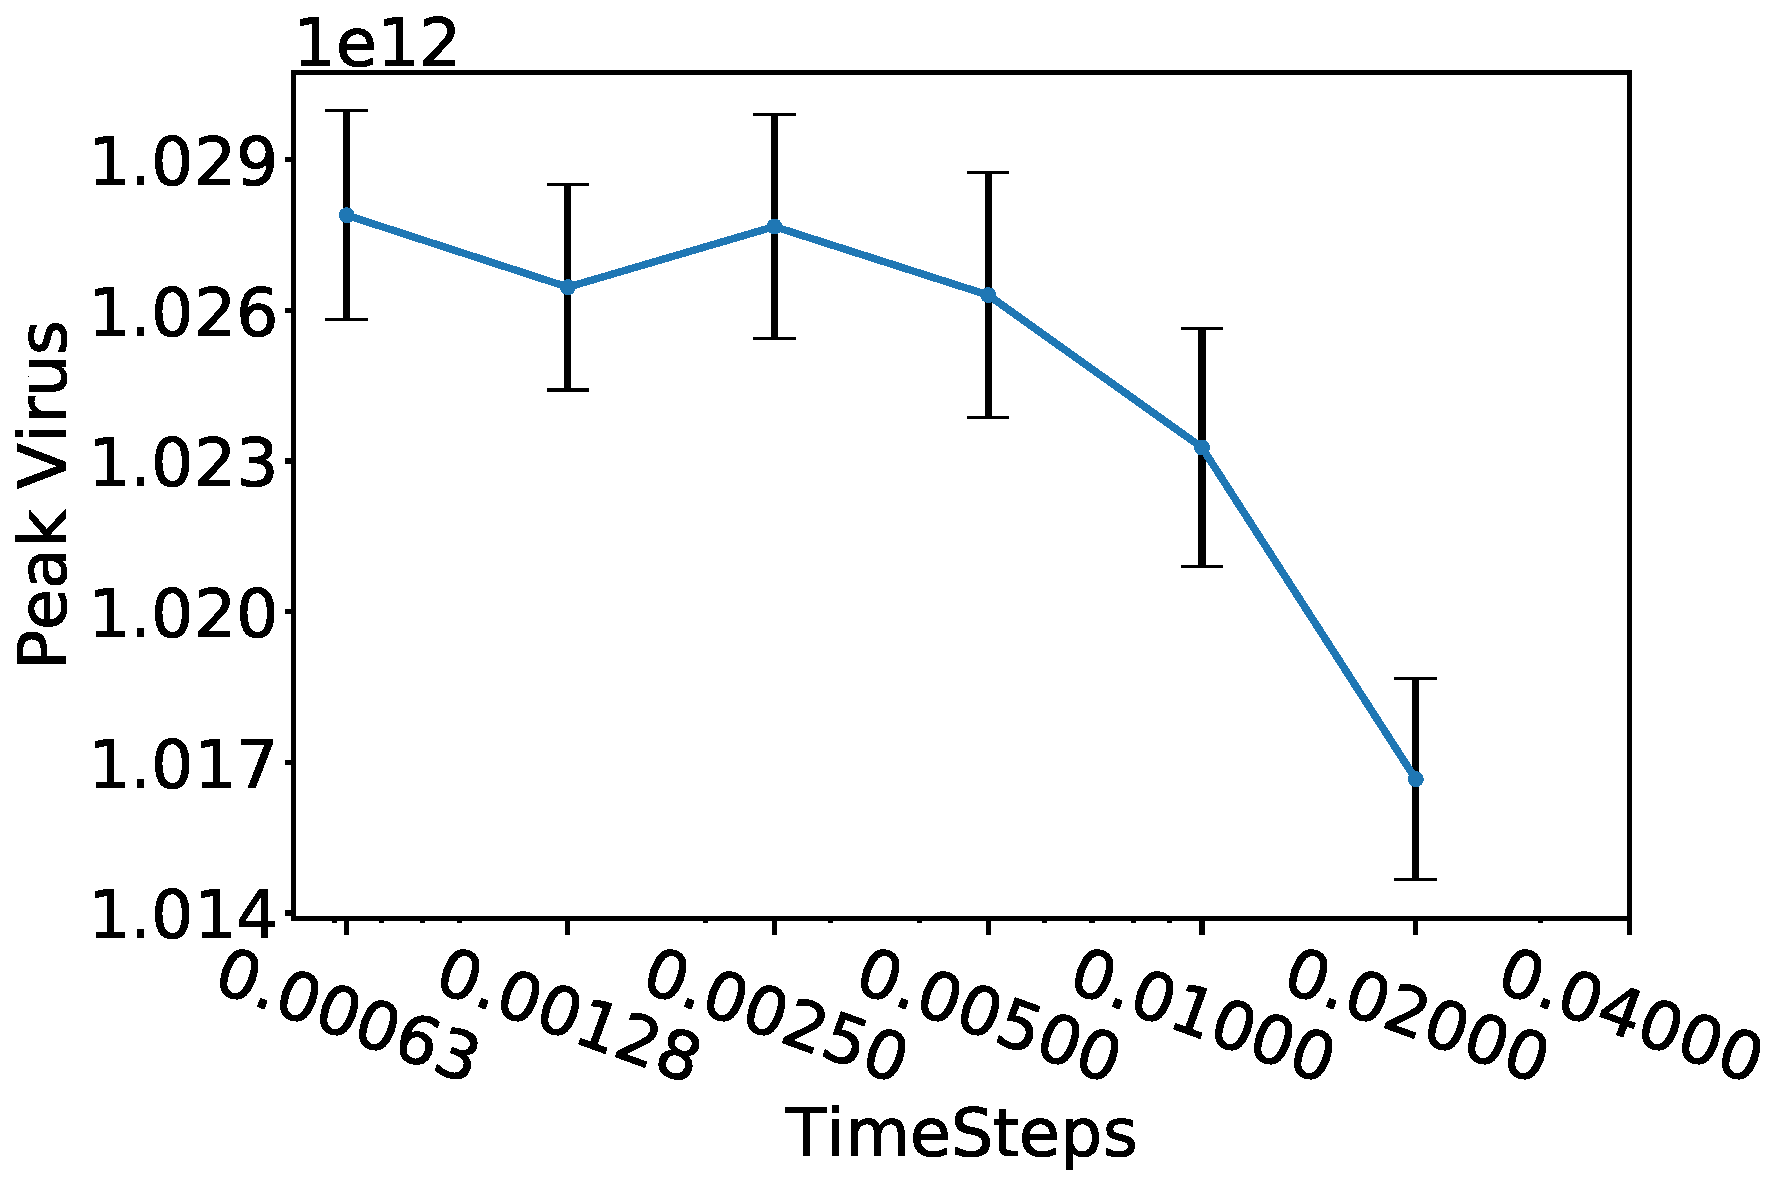
\includegraphics[width=0.33\linewidth]{Figures/Cellfree-InitialVirus-Runs_Graphs/PeakViralTiter.pdf}
    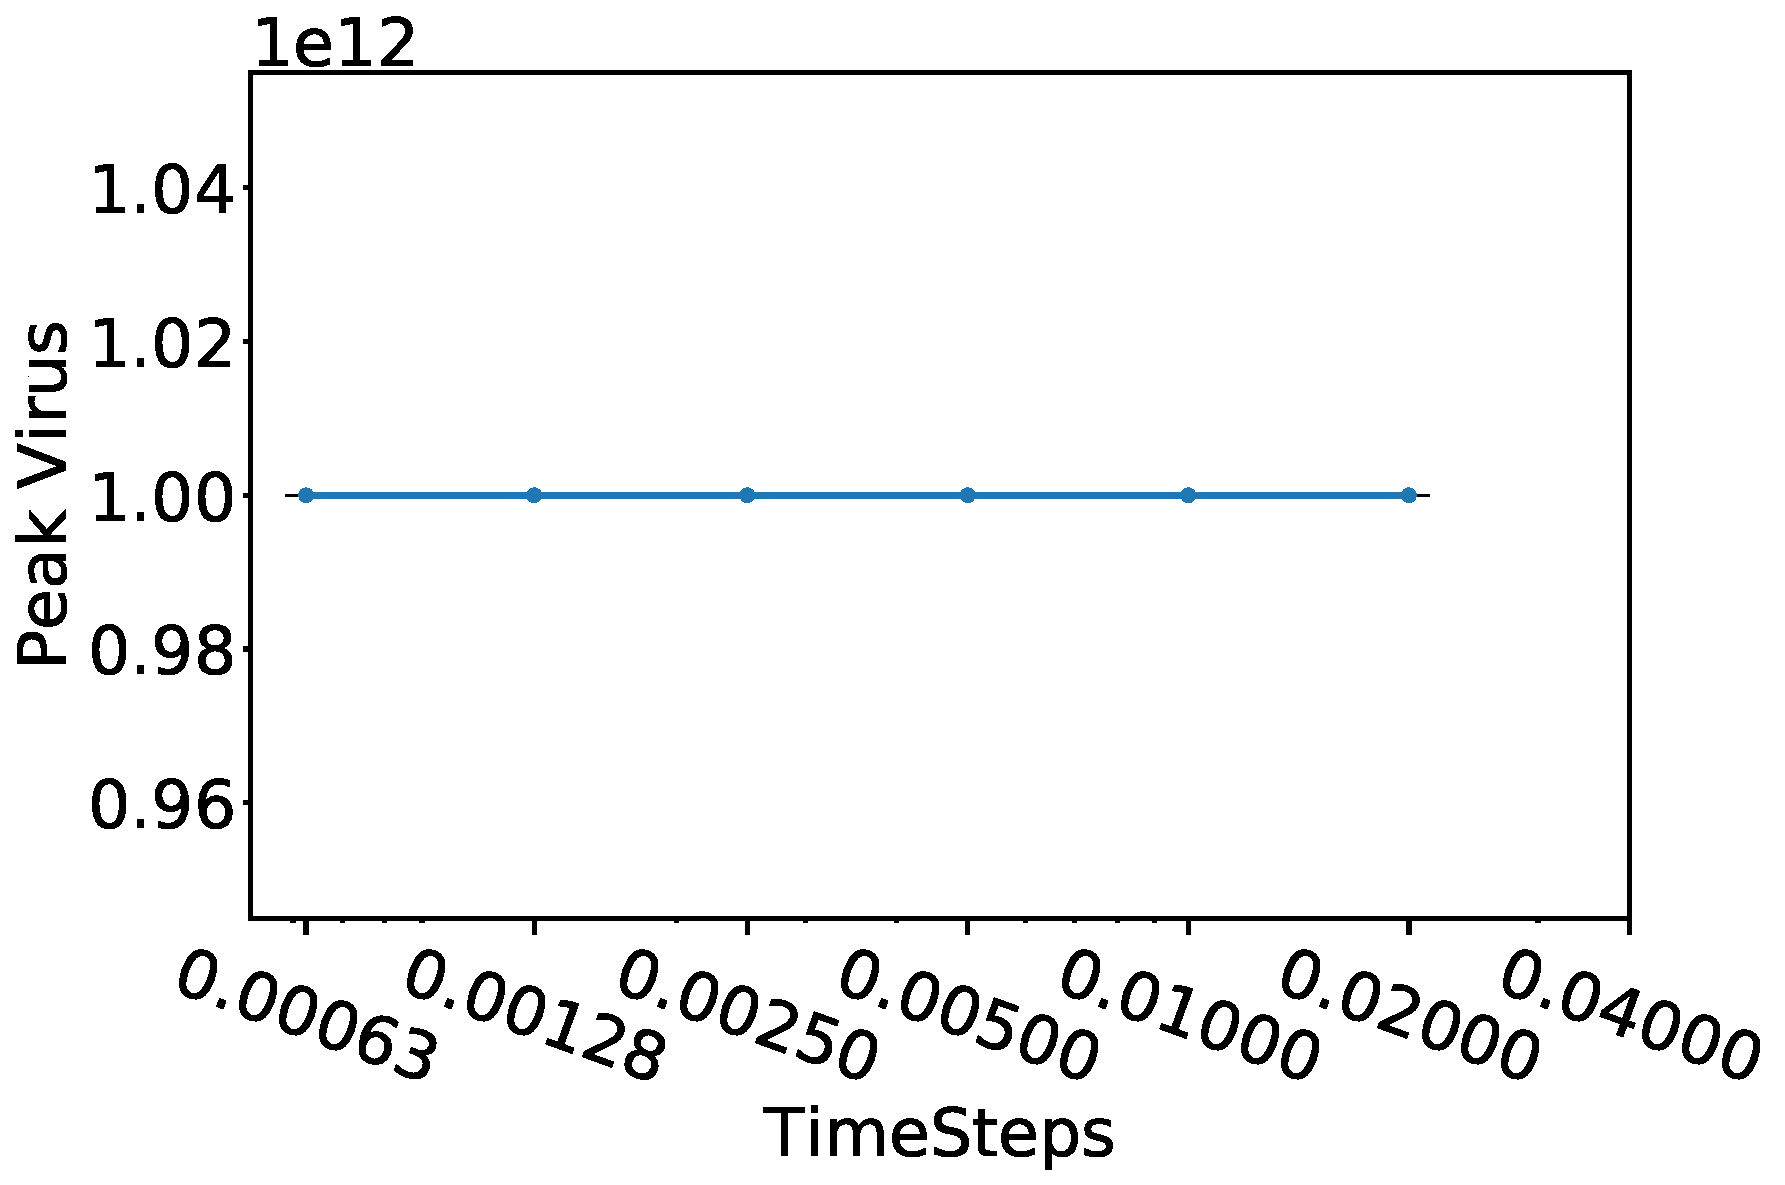
\includegraphics[width=0.33\linewidth]{Figures/Neither-InitialVirus-Runs_Graphs/PeakViralTiter.pdf}}

    \resizebox{\textwidth}{!}{%
    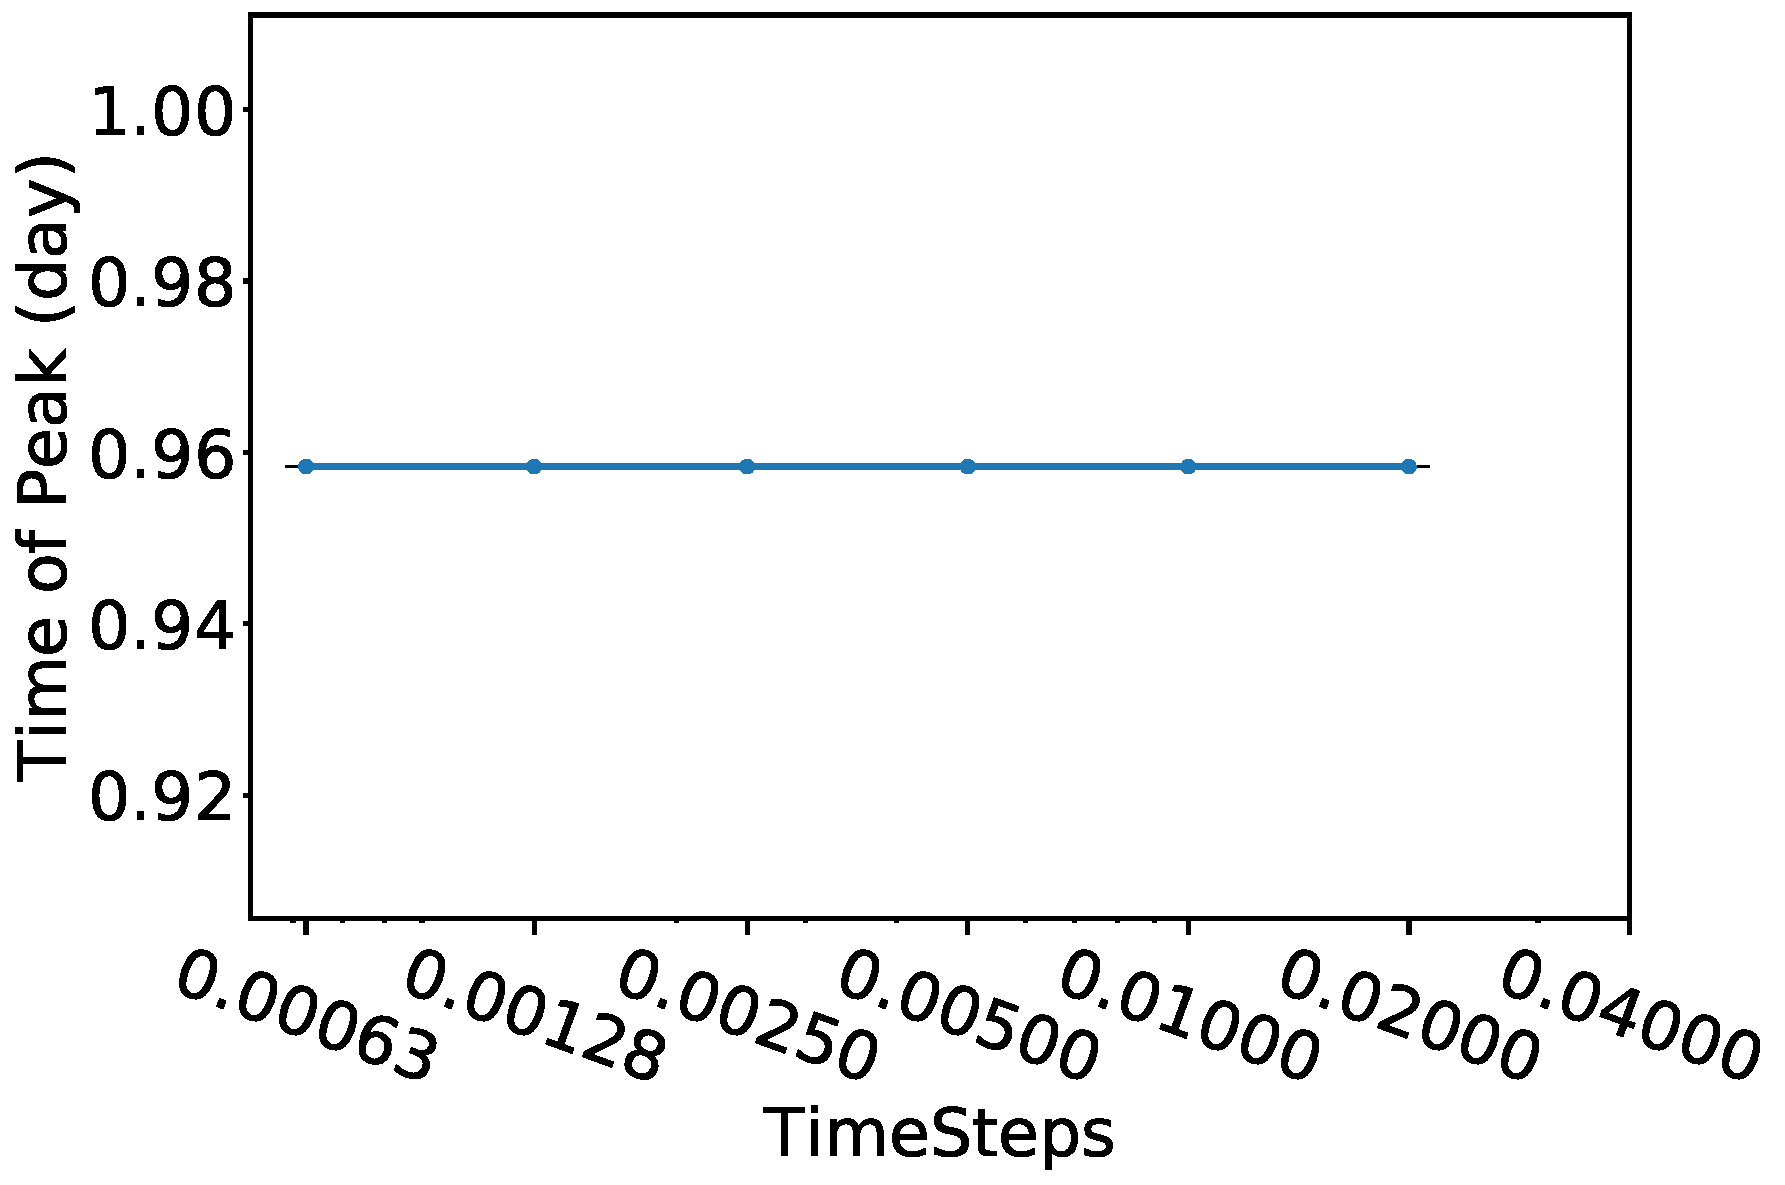
\includegraphics[width=0.33\linewidth]{Figures/Cellfree-InitialCell-Runs_Graphs/TimeofPeakViralTiter.pdf}
    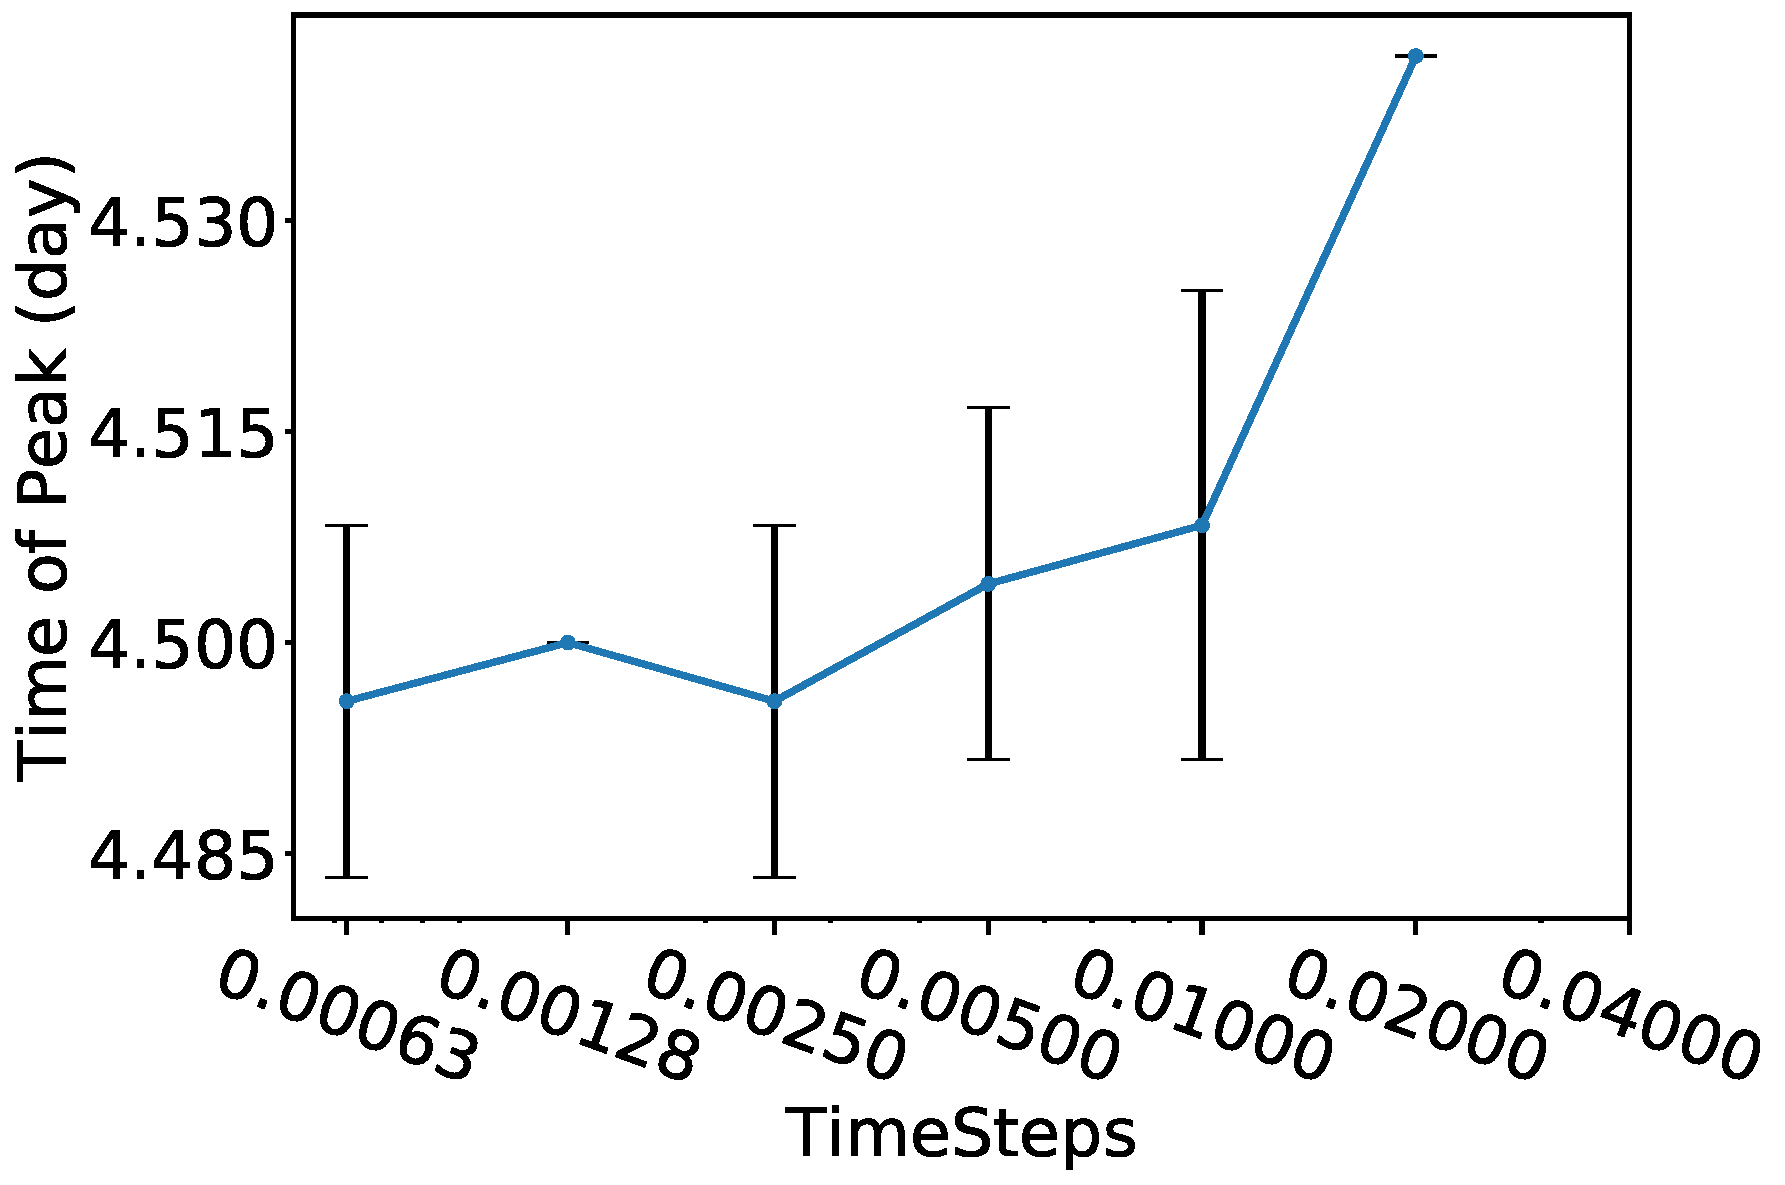
\includegraphics[width=0.33\linewidth]{Figures/Cellfree-InitialVirus-Runs_Graphs/TimeofPeakViralTiter.pdf}
    \includegraphics[width=0.33\linewidth]{Figures/Neither-InitialVirus-Runs_Graphs/TimeofPeakViralTiter.pdf}}

    \resizebox{\textwidth}{!}{%
    \includegraphics[width=0.33\linewidth]{Figures/Cellfree-InitialCell-Runs_Graphs/UpSlope.pdf}
    \includegraphics[width=0.33\linewidth]{Figures/Cellfree-InitialVirus-Runs_Graphs/UpSlope.pdf}
    \includegraphics[width=0.33\linewidth]{Figures/Neither-InitialVirus-Runs_Graphs/UpSlope.pdf}}}
\end{minipage}
\caption{Characteristics of the viral titer curves where measured for each of the seven time steps and the different scenerios.\label{fig_AspectGraphs}}
\end{figure}

\section{Fitting the model to data} \label{result_fit}

The model is fit to three experimental \emph{in vitro} data sets \citep{pinilla12} and \citep{wang_susceptibility_2021} via minimization of the SSR. For the \citep{pinilla12} data, the initial condition of the simulations were: 501535 cells in the dish (similar to the number of cells in a typical 24-well plate \citep{Number_of_cells_in_a_dish}), 250 initial infected cells, and no virus in the dish. On the left in figure \ref{fig_DataFit} is the median curve of ten simulations, using the best fit parameters, plotted in dark blue alongside the data in green. For both of the cell lines used from the \citep{wang_susceptibility_2021} data, the initial condition of the simulations were: 501535 cells in the dish (similar to the number of cells in a typical 24-well plate), 0 initial infected cells, and \num{5e4} virus in the dish. In the center and on the right of figure \ref{fig_DataFit} are the median curves of ten simulations, using the best fit parameters, plotted in dark blue alongside the data in green. The best fit parameters for each set of data are presented in table \ref{tab_datafit_params}.

\begin{table}
\centering
\caption{Best fit parameter values from fitting the model to experimental data \citep{pinilla12, wang_susceptibility_2021}. \label{tab_datafit_params}}
\resizebox{\textwidth}{!}{%
\begin{tabular}{llrrr}
\hline
 & & Pinilla et al.\ & Wang et al.\ Vero76 & Wang et al.\ Vero \\
Parameter & Meaning & Value & Value & Value \\
\hline
$\beta$ & Infection rate & \SI{54}{\per\hour} & \SI{56}{\per\hour} & \SI{69}{\per\hour} \\
$p$ & Viral production rate & \SI{3000}{\per\hour} & \SI{3.9}{\per\hour} & \SI{2.4}{\per\hour} \\
$c$ & Viral clearance rate & \SI{0.25}{\per\hour} & \SI{0.01}{\per\hour} & \SI{0.06}{\per\hour} \\
$D$ & Diffusion coefficient & \SI{2.2e-8}{\meter\squared\per\hour} (fixed) & \SI{1.7e-8}{\meter\squared\per\hour} (fixed) & \SI{1.7e-8}{\meter\squared\per\hour} (fixed) \\
$\tau_E$ & Mean eclipse duration & \SI{16}{\hour} & \SI{2.9}{\hour} & \SI{3.8}{\hour} \\
$\eta_E$ & Eclipse shape parameter & \num{30} (fixed) & \num{30} (fixed) & \num{30} (fixed) \\
$\tau_I$ & Mean infectious lifespan & \SI{26}{\hour} & \SI{17}{\hour} & \SI{18}{\hour} \\
$\eta_I$ & Infectious shape parameter & \num{100} (fixed) & \num{100} (fixed) & \num{100} (fixed) \\
\end{tabular}}
\end{table}

\begin{figure}
\centering
    \parbox{\textwidth}{
    \fbox{\parbox{\textwidth}{\vspace{-1em}
    \begin{multicols}{3}
        \centering

        Pinilla

        Wang Vero76

        Wang Vero
    \end{multicols}
    \vspace{-1em}}}

    \vspace{0.5em}
    \resizebox{\textwidth}{!}{%
    \includegraphics[width=0.33\linewidth]{Figures/Pinilla_DataFit.pdf}
    \includegraphics[width=0.33\linewidth]{Figures/Vero76_DataFit.pdf}
    \includegraphics[width=0.33\linewidth]{Figures/Vero_DataFit.pdf}}}
\caption{The ten simulated titer curves and corresponding median curve, from the fitting process, are plotted in blue. The experimental cell-free transmission data \citep{pinilla12} is plotted in green. The median curve has the minimal SSR with respect to the experimental data, when using the best fit parameters. The best fit parameters are shown in \ref{tab_datafit_params}. \label{fig_DataFit}}
\end{figure}

From the best fit parameters in table \ref{tab_datafit_params}, 100 simulations for each data set were produced. All one hundred runs and the median curve for each data set are shown in figure \ref{fig_FitRuns}. To showcase how the different parameters change the viral titer, the initial conditions of the simulated dish were the same for the different data sets. The initial conditions were: 1001365 cells in the dish (similar to the number of cells in a typical 35 mm petri dish), 500 initial infected cells, and no initial virus in the dish. It is easy to notice in figure \ref{fig_FitRuns} that the simulations of the Pinilla et al.\ data vary more than simulations of the Wang et al.\ data; this is from the change in standard deviation of the eclipse phase length of the cells. This will be discussed more in section \ref{findings} of the discussion chapter.

\begin{figure}
\centering
    \parbox{\textwidth}{
    \fbox{\parbox{\textwidth}{\vspace{-1em}
    \begin{multicols}{3}
        \centering

        Pinilla

        Wang Vero76

        Wang Vero
    \end{multicols}
    \vspace{-1em}}}

    \vspace{0.5em}
    \resizebox{\textwidth}{!}{%
    \includegraphics[width=0.33\linewidth]{Figures/Pinilla_AllOnOne.pdf}
    \includegraphics[width=0.33\linewidth]{Figures/Vero76_AllOnOne.pdf}
    \includegraphics[width=0.33\linewidth]{Figures/Vero_AllOnOne.pdf}}}
\caption{Using the best fit parameters in table \ref{tab_datafit_params}, a hundred simulated titer curves and corresponding median curve are plotted in purple. \label{fig_FitRuns}}
\end{figure}

\section{Summary}

In this chapter, I've shown that the model produces accurate simulations that compare to real experimental plaque assays and that the model can reproduce experimental data.


%%%%%%%%%%%%%%%%%%%%%%%%%%%%%%%%%%%%%%%%%%%%%%%%%%%%%%%%%%%%%%%%%%%%%%%%%%%



